\documentclass[12pt,preprint]{aastex}
%\documentclass[preprint]{aastex}

\usepackage[textwidth=0.8in,colorinlistoftodos]{todonotes}

%#For adding line numbers:
\usepackage{lineno}
\linenumbers


\usepackage{rotating}
\usepackage{amsmath}
\usepackage{graphicx}
\usepackage{xspace}
\usepackage{url}

% Note, hyperref has to come after other packages!
\usepackage{hyperref}

% some units
\newcommand{\mev}{\text{MeV}\xspace}
\newcommand{\gev}{\text{GeV}\xspace}
\newcommand{\tev}{\text{TeV}\xspace}
\newcommand{\sr}{\text{sr}\xspace}
\newcommand{\s}{\text{s}\xspace}
\newcommand{\ph}{\text{ph}\xspace}
\newcommand{\cm}{\text{cm}\xspace}
\renewcommand{\sec}{\text{s}\xspace}
\newcommand{\tsext}{{\ensuremath{\text{TS}_\text{ext}}}\xspace}
\newcommand{\tsinc}{\ensuremath{\text{TS}_\text{inc}}\xspace}
\newcommand{\loglikelihood}{\ensuremath{LL}\xspace}

\newcommand{\rsixeight}{{\ensuremath{\text{r}_{68}}}\xspace}

\newcommand{\tsextpointlike}{\ensuremath{\tsext_{,\pointlike}}\xspace}
\newcommand{\tsextgtlike}{\ensuremath{\tsext_{,\gtlike}}\xspace}
\newcommand{\tsextalt}{\ensuremath{\tsext_{,\alt}}\xspace}

\newcommand{\ts}{\text{TS}\xspace}
\newcommand{\glon}{\text{GLON}\xspace}
\newcommand{\glat}{\text{GLAT}\xspace}
\newcommand{\alt}{\text{alt}\xspace}

\renewcommand{\deg}{\ensuremath{^\circ}\xspace}

% the program names
\newcommand{\pointlike}{\text{\em pointlike}\xspace}
\newcommand{\python}{\text{\em python}\xspace}
\newcommand{\gtlike}{\text{\em gtlike}\xspace}
\newcommand{\gtobssim}{\text{\em gtobssim}\xspace}
\newcommand{\minuit}{\text{\em Minuit}\xspace}

\shorttitle{Search for Extended LAT Sources}

\begin{document}

\title{Search for Spatially Extended Fermi-LAT Sources Using Two Years of Flight
Data}

\author{
J.~Lande\altaffilmark{3}, 
\altaffiltext{3}{W. W. Hansen Experimental Physics Laboratory, Kavli Institute for Particle Astrophysics and Cosmology, Department of Physics and SLAC National Accelerator Laboratory, Stanford University, Stanford, CA 94305, USA}
}


\begin{abstract}
We present a new method for analyzing spatially extended sources with
the Large Area Telescope (LAT), the primary science instrument on the
{\em Fermi Gamma-ray Space Telescope (Fermi)}. Measuring the extension
of a LAT source is important for uniquely identifying it.  We provide
a series of Monte Carlo studies to validate this tool and calculate
the LAT's detection threshold to spatially extended sources.  We then
apply this tool to test all sources in the two year source catalog for
extension. We present on the detection of ten spatially extended sources
in addition to the twelve spatially extended sources reported in the
second Fermi LAT Catalog.
\end{abstract}

\listoftodos

\section{Introduction}

The Large Area Telescope (LAT) is a pair conversion telescope on the
Fermi Gamma-Ray Space Telescope (Fermi). It has been surveying the $\gamma$-ray
sky since June 2008.  Fermi is well suited as a survey
instrument because of its broad energy coverage (20 \mev
to $>300$ \gev), wide field of view ($\sim 2.4 \sr$), and large effective
area ($\sim 8000 \cm^2$ at $>1 \gev$).

Using one year of all sky surveying data, the LAT published a catalog of
source that were significantly detected.  Many of these were associated
with a variety of source classes including active galactic nuclei,
pulsars, galaxies, and supernova remnants.  Many of these classes can be
spatially resolved when observed at other frequencies and could possibly
be spatially resolvable in \gev by the LAT.

The LAT collaboration has previously reported on the discovered
a variety of spatially extended including the supernova remnants (SNRs)
IC443 and W51C (\cite{ic443,w51c}),
the pulsar wind nebulae (PWNe) MSH 15-52 and Vela X
(\cite{msh1552,velax}), and the Large Magellanic
and the Small Magalenic Cloud (\cite{lmc,smc}).  There are other
source classes which could possibly be spatially resolved by the LAT
including galaxy clusters, dark matter, and possibly new physics.

Furthermore, a variety of spatially extended but otherwise unassociated
sources have been detected in the galactic plane at \tev energies using
Air Cherenkov detectors. Most prominent was a survey of the galactic plane
using the High Energy Stereoscopic System (H.E.S.S) which discovered 14
spatially extended sources (\cite{HESS_plane_survey}).

Being able to spatially resolve the \gev emission from a source is
important for several reasons. Because of the large point spread
function (PSF), there are often several possible source counterparts.
Finding a matching morphology can be used to uniquely identify the source.
Because of the largely varying PSF of the LAT, the spatial and spectral
information about a source do not nicely decouple. Therefore, a biased
spatial model will bias the spectral model of the source and studying
the extension of the source can correct for this.  Furthermore, correctly
modeling a source's extension is important for improving the overall model
of the sky and removing excess residuals.  These residuals manifested
themselves in the one year catalog as spurious point sources in the
region region surrounding the Large Magellanic Cloud (\cite{first_cat}).


\section{Analysis Methods}

Morphological studies of sources in the \gev energy range
using the LAT are challenging because of the significantly 
energy-dependent PSF and because of systematic errors in the galactic diffuse
emission.  The LAT's PSF is determined at lower energies by multiple
scattering in the tracker and the 68\% containment radius of the PSF is
approximately 5.1\deg at 100 \mev  when averaged over instrument acceptance
and including photons which convert in either the thick or thin layers of
the tracker. The PSF approaches a limit given by the granularity of the
tracker channels and is 0.14\deg at 10 \gev (\cite{on_orbit_calibration}).
Therefore, the higher energy photons are significantly more important for
resolving a source but are typically limited by statistics. 
A detailed analysis procedure must be used to maximize our
sensitivity over all energies.

\subsection{The \pointlike Package}

A new analysis tool has been developed to address the unique requirements
for studying spatially extended sources with the LAT. The tool
provides a maximum likelihood analysis where the Poisson likelihood
for observing the measured counts is maximized by fitting
parameters of the model.  The extension of a source can be modeled by a
geometric shape (e.g. a disk or Gaussian) and the source's position
and extension can be simultaneously fit.

This analysis is not feasible using the official LAT likelihood
analysis tool \gtlike\footnote{\gtlike is distributed publicly by the
Fermi Science Support Center (\cite{fssc})} because \gtlike can only 
fit the spectral parameters of the model. The extension fitting would
have to be done as an external loop which would typically be
too time consuming. What has typically
been done to study an extended sources is to fix the position of the
source and develop a profile of the likelihood as a
function of extension.  This approach is not optimal because the
position and extension of the source should be simultaneously maximized
to find the best fit parameters and to correctly compute the statistical
significance of the detection.  Furthermore since this approach is
computationally intensive, no large scale Monte Carlo effort can
be run to validate it.

We developed an alternate approach to fit spatially extended
sources. A separate maximum likelihood fitting package called
\pointlike has been developed by the LAT collaboration and we have
added to it the ability to analyze spatially extended sources. \pointlike
is described in the one year catalog paper and in Matthew Kerr's Ph.D thesis
(\cite{first_cat,matthew_kerr_thesis}).  

What differentiates \pointlike most significantly from \gtlike is its
emphasis on speed by introducing approximations into the calculation
of the likelihood function while trying to minimized the introduced
numerical errors.  Like the binned version of \gtlike, \pointlike bins
the sky in both position and energy.  Unlike \gtlike, \pointlike relies on
the {\em healpix} representation of spatial bins (\cite{healpix}). Since
the PSF changes significantly with energy, the spatial size of each bin
is chosen to be smaller than the PSF. By changing the spatial
bin size with energy, \pointlike ensures that little information is lost
at each energy while minimizing the required number of bins.

\pointlike also bins $\gamma$-rays depending upon whether they convert
in the thin or thick layers of the tracker. Since the PSF is smaller for
photons which convert in the thin layers of the tracker,
photons are also binned depending upon where they 
convert in the tracker.
Furthermore, \pointlike
uses a sparse matrix representation of the spatial bins where only the
bins with counts in them are used. To evaluate the likelihood, \pointlike
then independently integrates the model predicted counts in the region.

Intelligent binning and a sparse matrix representation of the data
effectively interpolates between a binned analysis at low energy (where
the resolution is poor and there are many counts) and an unbinned
analysis at high energy (where the resolution is good but there are
few counts). This approach provides significant savings in time while
introducing only small numerical error.

\subsection{Extension Fitting}
\label{extension_fitting}

In \pointlike, it is assumed that the spatial and spectral model
of an extended source decouple and that the spatial shape can be
represented by a two dimensional function.  To fit the extended source,
\pointlike convolves the extended source shape with the PSF (as a
function of energy) and uses the \minuit fitting library to maximize
the likelihood by simultaneously fitting the position and extension
of the source (\cite{minuit_documentation}).  As will be described in
section~\ref{monte_carlo_validation}, simultaneously fitting the position
and extension is necessary to correctly calculate the statistical
significance of the detection of extension.  For each position and
extension, the spectral parameters of the sky model are refit. To avoid
projection effects, what is directly fit is not the longitude and latitude
but instead the source's displacement in a rotated reference frame.

The significance of the extension of a source can be calculated from
\tsext, which is defined as twice the increase in log likelihood (\loglikelihood)
between
the extended source model at its best fit values and the point source
model at its best fit values:
\begin{equation}
  \tsext=2\log(\loglikelihood_\text{ext}/\loglikelihood_\text{ps}).
\end{equation}
\pointlike calculates \tsext by fitting a source first with a spatially
extended model and then as a point source.  The interpretation
of \tsext in terms of a statistical significance is discussed in
section~\ref{monte_carlo_validation}.

The convolution of radially symmetric extended sources is optimized by
using a semi-analytic calculation.  The observed photon distribution
can be written as the convolution of the source shape ($I_\text{src}$)
with the psf
\begin{equation}
  \text{PDF}(\vec r) = \int  \text{PSF}(|\vec r - \vec r'|)I_\text{src}(\vec r') d A'.
\end{equation}
For the LAT, the PSF is parameterized as
\begin{equation}
  \text{PSF}(\vec r) = 
  \frac{1}{2\pi\sigma^2}
  \left(1-\frac{1}{\gamma}\right)
  \left(1+\frac{u}{\gamma}\right)^{-\gamma},
\end{equation}
where $\sigma$ and $\gamma$ are free parameters.  For radially symmetric
extended sources, the angular part of the integral can be done analytically
\begin{equation}
  \text{PDF}(u)= \int_0^\infty dv
  I_\text{src}(v) 
  \left(\frac{\gamma-1}{\gamma}\right)
  \left( \frac{\gamma}{\gamma + u + v}\right)^\gamma 
  \times ~_2F_1 \left(\gamma/2,\frac{1+\gamma}{2},1,\frac{4uv}{(\gamma+u+v)^2}\right).
\end{equation}
This convolution formula is used by \pointlike because it is faster
and more closely reduces to the PSF when the source's size is 
small.

\subsection{Extension Errors}
\label{extension_error}

Errors on fit parameters are typically calculated in one of two
ways. The first method requires explicitly varying a parameter
while simultaneously optimizing the other parameters
until the log of the likelihood has fallen by a particular value.
The \minuit fitting
package provides the {\em Simplex} function to calculate errors this way
(\cite{minuit_documentation}).  The second method involves estimating the
likelihood function as being a multivariate Gaussian and calculating the
curvature of the log of the likelihood at the peak to estimate when the
function will decrease by the desired value. \minuit provides the {\em HESSE}
algorithm to calculate errors this way.  {\em HESSE} errors 
can be calculated significantly faster.

We found that the {\em HESSE} errors on the extension of a source
were sometimes badly estimated.  On the other
hand, the {\em Simplex} algorithm was prohibitively slow and would often
fail to convergence. Our approach to calculating extension errors
is to fix the position of the source and varying just the extension
using the {\em Simplex} algorithm.  This approach
makes the approximation that the covariance between each spatial parameter
is small but not that the likelihood is Gaussian. This method 
is shown schematically in figure~\ref{extension_profile} which shows
the change in \loglikelihood when varying the extension of
the SNR IC443.
The localization error separately calculated by fixing the extension to the
best fit value and fitting an ellipse to the likelihood as a function
of the spatial parameters. This
elliptical localization error correctly accounts for the covariance
in the position of the source and this same me method is used to
calculate the localization error of all point sources in the first LAT catalog
(\cite{first_cat}).

\subsection{Gtlike Crosscheck}
\label{gtlike_crosscheck}

\pointlike is important for LAT analysis
that require many iterations such as source localization and extension
fitting.  On the other hand, we expect that the spectral parameters
fit by \gtlike to be slightly more precise.
Furthermore, because \gtlike is the standard likelihood analysis package,
it has been more extensively validated for spectral analysis.
For that reason, in the following analysis we took the best fit
position and extension found by \pointlike and
refit the spectral spectral parameters using \gtlike.
\gtlike also provides a second calculation of the likelihood which gives a
second measure of \ts and \tsext. We do not consider a source to be
significant unless there is agreement between the two methods.

We found good agreement between the two methods. For the new
extended source candidates, table~\ref{alt_diff_model_results} shows
a comparison of \ts and \tsext computed using \pointlike and \gtlike.
Unless explicitly mentioned, all \ts, \tsext, and spectral parameters
were calculated using \gtlike using \pointlike's positions and extensions.

\subsection{Dual Localization}
\label{dual_localization_method}

There is a degeneracy between a spatially extended source and multiple
point sources.  To assess the possibility of source confusion,
we developed a function in \pointlike to simultaneously fit 
the position of two point sources.
The code uses \minuit to fit the position of the two point
sources.  To avoid projection effects, the fit is done in a rotated coordinate
system.  To improve the robustness of the fit, Instead of directly fitting
the rotated coordinates $x_1$ and $x_2$ we instead
fit the sum and difference of the rotated
coordinates $S=(x_1+x_2)/2$ and $D=(x_2-x_1)/2$.  The \loglikelihood
is then maximized by fitting the sum and difference of the 
sources.  Because of \pointlike's computational efficiency, this algorithm
runs in a reasonable amount of time. 

We define \tsinc as twice the increase in \loglikelihood
fitting the region as two point sources compared to fitting the region
as one point source:
\begin{equation}
  \tsinc=2\times(\loglikelihood_\text{2pts}-\loglikelihood_\text{ps}).
\end{equation}
\tsinc can not be directly compared to \tsext to see which model is 
more significant
because the models are not nested (\cite{statistics_with_care}). Even
though the comparison of \tsext with \tsinc is not a calibrated test,
we find the extreme cases $\tsinc \loglikelihood \tsext$ or $\tsinc\gg\tsext$
to be suggestive and we only consider a source to be extended if
$\tsext>\tsinc$.

Like extended sources described in section~\ref{gtlike_crosscheck},
the spectrum of the two point sources can be refit using \gtlike. 
we quote the spectral values obtained from \gtlike using the best fit positions
found using \pointlike.  For the extended candidates found by our search,
we computed both \tsext and \tsinc.  The results are presented in
table~\ref{dual_localization_results}.

\subsection{Comparing Source Sizes}

\label{compare_source_size}

The spatial shape of extended sources can e modeled
as a two dimensional Gaussian
\begin{equation}
  \text{PDF}(x,y)=\tfrac{1}{2\pi\sigma^2}\exp\left(-(x^2+y^2)/2\sigma^2\right)
\end{equation}
or a uniform disk
\begin{equation}
  \text{PDF}(x,y)=\tfrac{1}{\pi\sigma^2}\delta\left(x^2+y^2<\sigma^2\right).
\end{equation}
Although these shapes are significantly different, the convolution
of them with the PSF for typical sizes look similar.  Even
though these shapes are significantly different, we demonstrate in
figure~\ref{compare_disk_gauss} that the convolution of shows the
PSF that would be observed for a power-law source of spectral index
2, the probability density function (PDF) for a Gaussian and uniform
disk of width $0.5\deg$, and the convolution of this PDF with the PSF.
The figure shows the convolution for the PSF in the energy range between
1 \gev and 100 \gev and also in the energy range between 10 \gev and
100 \gev.  The convolved shapes do separate better at higher energy, but
nevertheless this plot shows that we are not very sensitive to probing
the exact structure of an extended source.  In this paper we always
assume a uniform disk spatial model.

To get the convolved shapes to match in figure~\ref{compare_disk_gauss},
we had to set them to predict the same 68\% containment radius of 0.5\deg.  The
68\% containment radius for a spatial model is the radius at which 68\%
of the intensity is enclosed.  It can be computed by a straightforward
integral and we find that $\rsixeight_\text{,disk}=0.82\sigma$ whereas the
$\rsixeight_\text{,Gaussian}=1.51\sigma$.  Since $\rsixeight=0.5\deg$,
the uniform disk has $\sigma=0.41\deg$ whereas the Gaussian has
$\sigma=0.75\deg$.

This is important when comparing morphologies to other wavelengths
because the quoted size can vary significantly depending on which quantity
is reported.  This effect can be best seen in figure~\ref{compare_r68}
which a counts map of an extended source simulated in the energy
range from 1 \gev to 100 \gev with a uniform disk spatial model and
$\sigma=05$. Overlaid on the plot is the fit extension assuming the
source has a uniform disk and a Gaussian spatial model. The plot overlays
both $\sigma$ and $\rsixeight$ and $\sigma$ is significantly larger for
the disk spatial hypothesis compared to the Gaussian spatial model. On
the other hand, the disk and Gaussian's 68\% containment radius are
similar.

Since we are not very sensitive to the particular morphology of an
extended source, there is no correct choice for which size to quote
or which shape to overlay. For the following analysis, we quite the
disk's edge and overlay this size.  But due to smearing of the PSF,
$\sigma$ typically looks larger than the observed counts distribution.
When comparing the fit extensions with other wavelengths, it is important
to compare consistent quantities.


\section{LAT Extended Source Validation}


\subsection{Significance of Extension}
\label{monte_carlo_validation}

We validated \pointlike's extension fitting code with a Monte Carlo
study. \tsext (defined in section~\ref{extension_fitting}) can be used to calculate the statistical significance
of the extension of a source.  Since the point source and extended source models are
nested, an extended source must always fit as well as a point source.  On the other hand, we would
not expect the likelihood to change very much unless the source was
significantly extended.  Since an extended source has one additional
degree of freedom, Wilks' Theorem says that the distribution of $\tsext$
when testing a point source for extension should follow a $\chi^2_1$
distribution (\cite{wilks_theorem}).

On the other hand, since the null hypothesis rests on the edge of
parameter space when the extension is 0, Wilks' Theorem does not hold
(\cite{warn_wilks_theorem}).  One might expect the actual distribution
to be a half $\chi^2_1$ distribution with one degree of freedom plus
half a delta function at 0:
\begin{equation}
  P(\ts)=\tfrac{1}{2}(\chi^2_1(\ts)+\delta(\ts)).
\end{equation}
Chernoff proved that under certain assumptions this is the correct distribution
when the null hypothesis is on the edge of parameter
space (\cite{chernoff}).  The false detection
probability can be estimated by integrating this function from an observed
test statistic value to infinity. It is for this particular distribution
that the often quoted result holds that $\sqrt{\ts}$ is a measure of
the number of $\sigma$ of the detection (\cite{mattox_egret}).

The half $\chi^2_1$ distribution was found to hold for the special case
of source finding using EGRET (\cite{mattox_egret}). This distribution
is also plausible when testing point sources for extension. Due to
statistical fluctuations, half of the point sources might look narrower
than the PSF leading to $\tsext=0$. The other half of the time, we would
get a distribution consistent with Wilk's theorem. We will present a
Monte Carlo study that shows an empirical distribution of \tsext in the
null hypothesis and compares it to this distribution.

We simulated point sources of varying spectral models and fit them
them using \pointlike as both point and extended sources. The data was
simulated using \gtobssim\footnote{\gtobssim is distributed
by the Fermi Science Support Center (\cite{fssc}).}
The point sources were simulated with a power-law spectral model with
six $>100$ \mev fluxes ranging from $3\times 10^{-9} \ph/\cm^2/\sec$ to
$10^{-6} \ph/\cm^2/\sec$.  The point sources were simulated with spectral
indices ($\gamma$) of 1.5, 2, 2.5, and 3.  These values were picked to
to represent the types of sources detectable by the LAT.  The point
sources were simulated on top of an isotropic power-law background
with a Sreekumar-like spectrum ($>100$ \mev flux of $1.5\times 10^{-5}$ and spectral
index 2.1) (\cite{sreekumar_isotropic}).  The Monte Carlo simulation was
performed over a one year time interval using a default rocking profile
and a representative livetime fraction of 0.8.  The reconstruction was
performed with photons from an energy range of 1 \gev to 100 \gev using 4
energy bins per decade and using the 
Pass 7\_V6 (P7\_V6) Source Instrument
Response Function (IRFs).  For each point source, we used \pointlike
to fit it as both a point and extended source and calculate \tsext and
we only dept the sources which had a significant point source detection
($\ts>25$).

Before we present the results of the Monte Carlo simulations, we note
that despite out best efforts, there was always a small numerical
discrepancy between the likelihood when fitting the source as the PSF
and when fitting it as a very small extended source. This is due to
numerical error introduced by the convolution.  In most situations, this
error would be insignificant. But when testing a source for extension,
this offset significantly bias the distribution of \tsext in the null
hypothesis. To correct for this, instead of computing the likelihood in
the null hypothesis by fitting the PSF, we instead calculated \tsext by
fitting the sources as an extended source and as an extended source with
its extension fixed to ${10^{-10}}\deg$.

For most of the spectral models, ~30,000 statistically independent
simulations were performed. For the dimmer spectral models, many of the
simulations had $\ts<25$ and were discarded.  Table~\ref{ts_ext_num_sims}
shows the different spectral models used in our study as well as the
number of simulations.  The cumulative density of \tsext is plotted in
figure~\ref{ts_ext_mc}. The $\chi^2_1/2$ distribution suggested by Wilks'
Theorem is overlaid for comparison.

Our Monte Carlo study shows broad agreement between simulations and Wilks'
theorem. Nevertheless, the agreement is not perfect.  It should be noted
that the discrepancy seems to be worst for bright sources which seems to
imply that numerical errors in the convolution become more apparent for
sufficiently bright sources.  Other possible reasons for departure from
Wilks' theorem might include \pointlike ignoring energy dispersion which
would change the PSF's shape as a function of energy. But we emphasize
that most of the time, our empirical curve lies to the left of the
theoretical curve so using the theoretical distribution would lead to an
underestimate of the statistical significance of a detection. Therefore,
we are confident that $\sqrt{\tsext}$ can be used as a measure of the
statistical significance of a source's extension and use it in the
following analysis.

\section{Extended Source Detection Threshold}\label{extension_sensitivity}

We performed a second study to determine the LAT's detection
threshold to spatially extended sources. The detection threshold
to extension is defined as the flux at which the average
value of $\tsext$ is $\langle\ts\rangle=25$. As was seen in
section~\ref{monte_carlo_validation}, this corresponds to an extension
significance of $5\sigma$.  Qualitatively, we expect the LAT would not
be sensitive to sources much smaller than the PSF or much larger than
the PSF.  Small sources would look too much like the PSF and larger
sources would get lost in the background.

To calculate the LAT's detection threshold to spatially extended
sources, we simulated sources with a uniform radially symmetric disk
spatial model on top of a power-law Sreekumar-like isotropic spectrum
(\cite{sreekumar_isotropic}).  The Monte Carlo simulation was performed
using the same one year time interval as in section~\ref{monte_carlo_validation}.
For each extension and spectral index, we
first picked a flux range which bracketed $\tsext=25$. We then picked
ten flux points in this range and repeatedly simulated and performed
extension tests of the extended sources.  For each flux, we performed
$>15$ independent simulations and extension fits.  We calculated
$\langle\tsext\rangle=25$ by fitting a line to all the flux and
$\tsext$ values and estimating the flux when $\tsext=25$.

Figure~\ref{index_sensitivity} shows the threshold for sources of four
spectral indices from 1.5 to 3 and extension varying from $\sigma=0.1\deg$
to $2.0\deg$.  The curves on the plot represent the flux for a given
extension where $\langle\tsext=25\rangle$.  The plot shows the threshold
using photons with energies between 100 \mev and 100 \gev and the
threshold using only photons with energies between 1 \gev and 100 \gev.
This results shows that the LAT's threshold to extension is better for
harder sources with more high energy photons. This result also shows
that the threshold is best for sources with an extension of $~0.5\deg$
and is significantly worse for very small extended small.

Except for the hardest and largest sources, our detection threshold
is almost unchanged when using events between 100 \mev and 1 \gev.
This is also demonstrated in figure~\ref{ts_ext_vs_energy} which shows
the \tsext for the SNR IC443 computed independently in 12 energy bins between 100 \mev and
100 \gev. For IC443, which has a spectral index ~2.4, almost the entire
increase in \ts comes from energies above 1 \gev.  On the other hand,
other systematic errors become increasingly important at low energy. For
our extension search, we use only only photons with energy above 1 \gev.

Figure~\ref{diff_factor_sensitivity} shows how the LAT's detection
threshold varies with increasing diffuse background. We compute the
sensitivity for a power-law source of spectral index 2 using 1, 10, and
100 times the extragalactic background. The latter factor approximately
represents the intensity of the galactic diffuse emission near the
galactic center.  The figure shows two plots, the first showing the
threshold using only photons with energies between 1 \gev and 100 \gev and
the second showing the threshold using only photons with energies between
10 \gev and 100 \gev. This plot demonstrates that we are less sensitive
to extended sources in a higher background region and that if the flux of
a source is constant (same number of photons), we would be more sensitive
to the extension of that source if those photons had a higher energy.

\section{Extended Source Search Method}


The first and second LAT catalog produced a list of all significant point
sources seen by the LAT.  (\cite{first_cat,second_cat}).  The first LAT
catalog's source finding method assumes that all sources were consistent
with the PSF. The second LAT catalog modeled previously published
spatially extended sources with an extended spatial model but did not
attempt to resolve new spatially extended sources. In this paper,
we took the sources from the second Fermi LAT catalog and perform
a search to attempt to spatially resolve new sources.

For this search, we build a model of the
sky consistent with the second catalog.   We used the same two
years of data from August 4, 2008 to August 1, 2010 and we used the same
Pass 7\_V6 (P7\_V6) Source class event selections and 
Instrument Response Functions (IRFs, \cite{lat_on_orbit_psf}).  We used the same galactic diffuse,
isotropic diffuse, and earth limb emission model. The spectrum of the
galactic and isotropic diffuse models were refit during the analysis
while the earth limb emission was fixed to it's predicted value.

As was shown, we gain little in sensitivity using photons with energies
below 1 \gev. On the other hand, the large PSF at low energy makes us
more susceptible to systematic errors arising from source confusion due
to multiple point sources and susceptible to incorrect modeling of the
galactic diffuse emission.  For that reason, we performed our search
using photons only between 1 \gev and 100 \gev.
We used 4 energy bins per each logarithmic decade in energy.

We also performed a search for extended sources using photons only between
10 \gev and 100 \gev. Even though we are testing the same sources, this
approach is complimentary because there are regions in the galactic
plane where at lower energies the diffuse emission dominates and the
analysis is challenged by the difficulty in modeling this emission.
The analysis is also challenged by source confusion in crowded regions.
On the other hand, at the highest energies accessible by the LAT, the
galactic diffuse emission is less dominant and nearby sources might
be expected to be softer.  Using higher energies, we might expect
to detect harder sources in more complicated regions. This approach
is This is especially beneficial for regions near pulsars which
cutoff before 10 \gev.  This approach of using high energies was was
successfully used to detecting HESS J1825-137 and MSH 15-52 with the LAT
(\cite{msh1552,fermi_hess_j1825}).

For each catalog source, we tested it for extension using \pointlike
assuming the source had a uniform radially symmetric disk spatial model.
we used a circular $10\deg$ region of interest centered on our source and
included all catalog sources within $15\deg$ of the source of interest.
We refit the spectral parameters of sources within $2\deg$ of our source.
We modified the spectral index of each source we were testing to be a
power-law. This was reasonable because for a source to be significantly
extended, it would have to be fairly hard and fit reasonably well by
a power-law. Second, since we began our analysis at either 1 \gev or
10 \gev, we didn't expect there to be significant curvature over this
smaller energy range.

Finally, when analyzing our region, we automatically removed other
catalog sources which were within 0.5\deg of the source of interest. This was done because of
a concern that extended sources would end up in the catalog as
multiple point sources. These spurious catalogs sources would then
distort the extension fit.
For each extended candidate, we performed a dual localization procedure
(described in section~\ref{dual_localization_method} to test if the
source was extended multiple point sources.


\subsection{Additional Analysis}

We then selected all of the
sources for which \pointlike found $\tsext>16$.

We expect most extended sources to be inside the galactic plane
since extragalactic sources are typically too far away to be
resolvable. Unfortunately, the \gev emission in the galactic plane
is dominated by anisotropic galactic diffuse emission.  Modeling the
galactic diffuse emission and finding sources on top of this emission is
difficult (\cite{first_diffuse_paper}). This issue has been discussed in the
Fermi catalog (\cite{first_cat,second_cat}). Furthermore, the galactic plane is
crowded and so it is often difficult to get a good model for the
region around a catalog source.  Because of this, finding a source with
$\tsext>16$ is not a sufficient test and we perform several crosschecks
to ensure our overall region is well modeled.

% 2FGL J1856.2+0450c = P72Y3047 for
As an example of why this issue, we describe our test of 2FGL
J1856.2+0450c for extension.  Figure~\ref{example_bad_fit} shows
a smoothed counts map using photons with energy above 1 \gev. In
the map, the galactic and isotropic diffuse emission subtracted.
A two year catalog source 2FGL J1856.2+0450c was found at the position
$(l,b)=(37.79\deg,1.14\deg)$.  We find that there appears to be overall
some large scale residual in the diffuse emission along the galactic
plane. Furthermore, it appears that we don't have a great model of
the nearby catalog sources. As a result, 2FGL J1856.2+0450c fits to a
large extension of 1.37\deg and the result is statistically significant
with \tsext=51.6.  By looking at the residuals, it is clear that this
complicated region is not well fit even though the source's extension is
statistically significant. For this reason, we have to perform a series
of further analysis for all of the sources that are found with \tsext=16.
% information came from
% /nfs/slac/g/ki/ki03/lande/extended_catalog/2FGL/v15/standard_analysis/spectral_emin_1000_v1/P72Y3047/v1/results_followup_P72Y3047.yaml

First, we took the spatial and spectral model found using \pointlike
and performed a crosscheck by refitting the spectral parameters using
\gtlike.  We used a square ROI $14.1\deg$ in diameter with $1/16\deg$
pixels and the same energy binning. We found that $1/16\deg$ bins were
fine enough for \gtlike to get an extension significances consistent
with \pointlike.  Using \gtlike, we found a second measure of \tsext and
we only considered a source to be significantly extended if \pointlike
and \gtlike both agreed.  For the new extended source candidates, with
table~\ref{alt_diff_model_results} shows a comparison of their the value
of \tsext found by \gtlike and \pointlike.  Everywhere else, the values
from \gtlike are used.

Additionally, we generated for each extended source candidate residual
test statistic (\ts) maps.  The residual \ts map is a map of the \ts
value evaluated at each point by adding onto the map at that position a
new source of spectral index 2 and finding the increase in likelihood
when fitting its flux. \ts maps are especially useful as looking for
new sources or other residual features that are not included in the
model. They also have the advantageous feature that the absolute scale
can be used to clearly look for when the residual is significant.
The downside is they are biased to look for residual features that
look like the PSF and so are not as sensitive to diffuse residual
features. Furthermore, since by definition \ts>0, \ts maps can only show
positive fluctuations. Nevertheless, \ts maps were useful for assessing
the overall quality of the fit. Figure~\ref{res_tsmaps} shows an example
residual \ts map for the extended source IC443.


For each candidate, we also generated counts slices. A counts slice
plots the sum of all counts in the longitudinal direction within 2\deg
in the latitudinal direction.  The same plot is also shown integrating
in the longitudinal direction.  On top of the plot is overlaid the model
predicted counts assuming the source has a disk spatial model, assuming
the source is a point source, and fitting just the diffuse emission in
the region.  An example counts slice is shows for the extended source
IC443 in figure~\ref{counts_slice}. Counts slices were especially useful
for looking at how well the overall diffuse emission model fits the
region near the sources.

For each candidate, we also made was a radial integral of the data. This
plot shows the sum of all counts within a given distance from the
source's center. The plot is binned uniformly in $\Delta \theta^2$ so
that an isotropic background will be flat in the plot. On top of this
plot is overlaid the model predicted counts assuming the source has a
disk spatial model, assuming the source is a point source, and fitting
just the diffuse emission in the region. An example radial integral
is shown for the extended source IC443 in figure~\ref{radial_profile}.
This plot is best for comparing the observed counts to the PSF.

For each source, we computed an extension profile.  An example
extension profile for the extended source IC443 is shown in
figure~\ref{extension_profile}.

Finally, for each source, we performed the dual localization method
described in section~\ref{dual_localization_method}.  We did so by
replacing the source with two sources each containing half of the original
flux and then using \pointlike to simultaneously fit the position and
spectrum of these sources.  We then used \gtlike to refit the spectrum of
these sources using the best fit positions. For the new extended sources
found, we summarize the results of this dual localization test and compare
the values of \tsext to \tsinc in table~\ref{dual_localization_results}.

Because of the high source density in the galactic plane for promising
extended source candidates we often had to iteratively improve our model
of background sources to obtain a good fit of the extended source.
Often, several catalog sources would fill in the emission of one
extended source and all but one of them would have to be removed from
the model. Similarly, the position of background sources would often
have to be refit once the extended source's extension was correctly
fit. Similarly, background sources were insignificant in the fit energy
range and had to be removed.  When the localization of background
sources and the extension of our catalog source coupled, we iteratively
fit the position and extended of the nearby sources in the region until
the fitter stabilized on the overall best fit positions and extensions.
For each extended source, we describe what modifications were required
to the sky model to obtain a good fit of the region.

\subsection{Alternate Diffuse Model Crosscheck}
\label{alt_diff_model_description}

To estimate systematic errors due to uncertainty in our diffuse
emission background model, we performed a second
extension test of our candidates using
an alternate diffuse
model. Our alternate model was based on the GALPROP\footnote{GALPROP
is a software package for calculating the Galactic $\gamma$-ray
emission based on a model of cosmic-ray propagation in the Galaxy. See
\url{http://galprop.stanford.edu/} for details and references} code
used in the LAT analysis of the isotropic diffuse emission
(\cite{isotropic_lat}).  
With this model,
we independently fit in the nearby region 
7 HI rings, 7 HII rings, the inverse component,
the E(B-V) residual, and the isotropic component of
the background ration.
All told, we fit in or region 18 individual templates along
with all source parameters during the analysis.

It is not expected that this diffuse model is more physical.
But adding degrees of freedom to the background model is a good
way to remove additional degrees of freedom to the background
model is likely spurious sources which correlate to features in
the diffuse emission.  Therefore, this tests systematics that may
be due to incorrect modeling of the diffuse emission in the region.
The results of this fit for the new extended source candidates are shown
in table~\ref{alt_diff_model_results}. Overall, there is good agreement
between the \ts using the standard and alternate diffuse models.


\section{Validation of Known Extended Sources}
\label{validate_known}

We first present on our analysis of the twelve extended sources
previously published and include in the second catalog's sky model.
(\cite{second_cat}).


% 6 SNRs
The largest population of extended source are SNRs. The six
extended SNRs included in the second catalog are IC443, W28, W30,
W44, W51C, and the Cygnus Loop. These sources were first reported in
(\cite{ic443,w28,w44,w51c}).  Detailed papers studying W30 and the Cygnus
Loop are still in preparation.  Using photons with energies between 1
\gev and 100 \gev, our analysis significantly detected the extension
of all six SNRs. Table~\ref{known_extended_sources} shows the best fit
positions and extensions of these sources.


% 2 galaxies

Two galaxies the Large Magalenic Cloud and the Small Magalenic Cloud 
were included in the second catalog (\cite{lmc,smc}).  

% 3 PWN
Three pulsar wind nebula Vela X, MSH 15-52, and HESS J1825-137 were
included in the second catalog (\cite{velax,msh1552,fermi_hess_j1825}).
Using photons with energy above 10 \gev, we significantly detected the
extension of HESS J1825-137.  To improve our model of this source, we
removed the nearby catalog source 2FGL J1823.1-1338c which is part of the
extended emission of HESS J1825-137.  Using photons with energies above
10 \gev, we fit the extension of MSH 15-52 consistent with the published
result at an extension significance of \tsext=9.5.  Our analysis was
unable to resolve Vela X. An analysis of this source requires removing on
pulse events from the Vela pulsar and is beyond the scope of this paper.

\todo[inline]{note about how MSH 15-52 can't go lower in
energy because of nearby pulsar.}

% 1 radio galaxy
Centarus A.

Our analysis also failed to detect a significant extension for the
Centaurus A Lobes (\cite{cen_a_lat}). This is most likely because the
discovered emission was significantly more complicated then a uniform
radially symmetric Disk.  

The results are summarized in table~\ref{known_extended_sources}.
This table includes the best fit position and extension of these
sources when fitting them with a radially symmetric uniform disk spatial
model.  It also includes the best fit spectral model of each source.
The difficulty our analysis analysis had fitting the extension of several
of the already published extended sources should be used to emphasize
the overall difficultly in studying spatially extended sources in crowded
regions of the sky.

\section{Test of 1LAC Sources}
\label{test_1lac_sources}

To validate our method and assess systematic issues with our analysis,
we used \pointlike to test known active galaxies (AGN) for extension.
\gev emission from AGN is believed to comes from the core of supermassive
blackholes in small regions in the core of distant galaxies.  AGN are
not expected to be spatially resolvable and therefore provide a good
calibration source to demonstrate the efficacy of our tool. Nevertheless,
it would be interesting if AGN could be spatially resolved and
there are theories that predict this (\cite{pair_halo_paper}).

Following the LAT's one year catalog, the LAT collaboration published
a list of catalog sources that had a high probability association with
AGN (\cite{first_agn_cat}).
The first year catalog had 709 AGN associated with 671 distinct
1FGL sources at high latitude ($|b|>10\deg$).  To avoid systematic
problems with AGN classification, we used only the 599 AGN which made
it into the clean AGN sample.  An AGN association is only considered
clean if it has a high probability of association $P\ge 80\%$, if it is
the only AGN associated with the 1FGL source, and if there are no flags
on the catalog source (\cite{first_cat}). These last two conditions are
especially important for our analysis.  Source confusion may look like
a spatially extended source and flagged catalog sources may correlate
with unmodeled structure in the diffuse emission.

Of the 599 ``clean'' AGN, we select 556 of these 1FGL sources which
we uniquely associate with a 2 year catalog source. We furthermore
restrict our select to the 515 of these AGN for which we fit $\ts>25$
using \pointlike and photons with energy above 1 \gev.  Our intention
here is not to find the largest sample of AGN but simply
to find a goog sample to test the systematics of our extended source
search.

Using the same extension fitting procedure as described above, we tested
these 515 AGN for extension. A histogram of the \tsext values computed
with \pointlike is shown in figure~\ref{agn_ts_ext}. Overlaid on the plot
is a $\chi^2/2$ distribution suggested by Wilks' Theorem.  This plot
shows a worse agreement with the theoretical distribution and
a discrepancy with 
our Monte Carlo study in figure~\ref{ts_ext_mc}.  But overall, the
distribution is good. No AGN get fit with a particularly significant
value of $\tsext$ and almost all of the AGN get fit with $\tsext<1$.
There where only two AGN with $\tsext>10$. The maximum had $\tsext=13.7$
whereas the maximum value expected theoretically by the $\chi^2/2$ distribution is
8.3. This result shows that there is some systematic with our
analysis but that it will not significantly affect our analysis.
% 8.3 number gotten from mathematica:
% PDF[ChiSquareDistribution[1], x]
% N[Solve[(1/2)*
%     Integrate[1/(E^(x/2)*(Sqrt[2*Pi]*Sqrt[x])), {x, TS, Infinity}] &=&  
%        1/515, TS]]

Several possible systematics could cause this discrepancy. The first is
that in our analysis we fit each source with a power-law spectral model.
AGN tend to have curved spectral and fitting with the wrong spectral
model might effect the value of \tsext. Nevertheless, since we use only
photons with energy above 1 \gev, this effect is not expected to be large.
Another possible source for the discrepancy is that \pointlike performs
a likelihood analysis without modeling the energy dispersion of the LAT.
This probably is not the cause because energy dispersion is expected to
be more significant at low energy and it would have also showed up with
the Monte Carlo simulations.

Another possible systematic may be due to source confusion to problems
with the background model. If the two sources were close, they may
be unresolvable and get fit as a more significant extended source.
It is also possible that there are lingering residuals in the diffuse
emission. Unmodeled parts of the diffuse emission could be filled in by
modeling point sources as being slightly extended.

The final effect that could cause this discrepancy is an imperfect
modeling of the PSF.  Before launch, the PSF
was determined by a Monte Carlo simulation of the detector.
After launch, a discrepancy was found using flight data above a
few \gev in the PSF measured using bright AGN.  This result
was presented in conference and a publication is in preparation.
Subsequently, the PSF was fit empirically to bright AGN and this
empirical parameterization was used in our instrument
response function (\cite{lat_on_orbit_psf}).
But our current parameterization is not perfect. There are lingering
issues due to a lack of statistics at high energy which makes it hard to
validate the PSF as a function of the incident angle of the photon. Since
the distribution of incident angles varies from source to source, an
average PSF may make some of the sources look more and less extended
than the PSF.

We should finally clarify that since the PSF was found empirically
from the shape of bright AGN, finding that the AGN we test are not
significantly extended is not surprising.  All this analysis shows
is that the we can significantly find sources larger than bright AGN
found by the LAT.  Trying to look for the extension of these AGN as a
population would require a more specialized analysis.

\section{New Extended Sources}
\label{new_ext_srcs_section}

% Notes about extended Catalog sources
% Catalog used for analysis is P72Y_uw23.fits
% Compare to final catalog gll_psc_v04.fit
%          1FGL Name - Preliminary 2FGL - 2FGL Name
% 1FGL J1628.6-2419c - P72Y2516         - 2FGL J1627.0-2425c
% 1FGL J1554.0-5345c - P72Y2405         - 2FGL J1554.4-5317c
% 1FGL J0823.3-4248  - P72Y1212         - 2FGL J0823.0-4246
% 1FGL J1711.7-3944c - P72Y2674         - 2FGL J1712.4-3941

% 1FGL J1613.6-5100c - P72Y2472         - 2FGL J1615.0-5051 
% 1FGL J1614.7-5138c - P72Y2473         - 2FGL J1615.2-5138
% 1FGL J1632.9-4802c - P72Y2540         - 2FGL J1632.4-4753c
% 1FGL J2020.0+4049  - P72Y3281         - 2FGL J2021.5+4026
% 1FGL J1837.5-0659c - P72Y2974         - 2FGL J1837.3-0700c
% N/A                - P72Y1287         - 2FGL J0851.7-4635

Ten extended sources not include in the second LAT catalog were found
using this search.  Four were found in our search using only photons
with energies above 1 \gev and six were found only using photones with
energies above 10 \gev.  The fit properties of these ten sources is
summarized in table~\ref{new_ext_srcs_table}.  The table includes for each
source the best fit position, extension, spectrum, source significance,
and significance of extension.  Figure~\ref{allsky_extended_sources}
shows a skymap of the position of the twelve sources included in the
second catalog and the ten sources analysis in this paper.

For all the extended sources, table~\ref{dual_localization_results}
presents information about the of source confusion by fitting the same
region as two point sources using the dual localization method described
in section~\ref{dual_localization_method}. The table compares \tsext
to \tsinc and summarized the positions and spectra of the two sources.
Finally, table~\ref{alt_diff_model_results} summarized the results of
a crosscheck of the source fitting the region with an alternate diffuse
model described in section~\ref{alt_diff_model_description}.  These tables
show that our extended sources are not likely the result of source confusion
and that they are robust to changing the diffuse emission model.


\subsection{2FGL J0823.0-4246}
\label{section_2FGL_J0823.0-4246}

% 1FGL J0823.3-4248  - P72Y1212         - 2FGL J0823.0-4246
% Deleted 
%  * P72Y1214 - 2FGL J0823.4-4305
%  * P72Y1210 - 2FGL J0821.0-4254

The two year catalog source 2FGL J0823.0-4246 was found to be
extended using photons with energy between 1 \gev and 100 \gev.
We found an extension of $0.37\deg\pm0.03\deg$ and an extension
significance of $\tsext=46.1$.  The source was fit to a position of
$(l,b)=(260.32\deg,-3.28\deg)$.  Figure~\ref{1FGL_J0823.3-4248} shows a
counts map of this source.  This source is coincident with the one year
catalog source 1FGL J0823.3-4248.

To get a good fit of the source, we had to remove the nearby catalog
sources 2FGL J0823.4-4305 and 2FGL J0821.0-4254 which are part of the
extended emission.  We tested the source for source confusion by fitting
it as two point sources. Because $\tsinc=21.9$ is smaller then \tsext,
we conclude that this is an extended source.  
These modifications are shown in
figure~\ref{1FGL_J0823.3-4248}.

This extended source is spatially coincident with the SNR Puppis A.
Overlaid on figure~\ref{1FGL_J0823.3-4248} are ROSAT contours of Puppis
A (\cite{rosat_puppis_a}). There is good agreement between of the X-ray
shape with the fit size in \gev.

\todo[inline]{Add interpretations of Puppis A}

\subsection{2FGL J1627.0-2425c}
\label{section_2FGL_J1627.0-2425c}

% 1FGL J1628.6-2419c - P72Y2516         - 2FGL J1627.0-2425c
% No modifications to background were needed

The two year catalog source 2FGL J1627.0-2425c was found to be
significantly extended when using photons with energies between 1 \gev
and 100 \gev.  The best fit extension was $0.53\deg\pm0.06\deg$ and the
best fit position is $(l,b)=(352.87\deg, 16.79\deg)$.
The extension significance was $\tsext=20.3$. 
This source is coincident with the one year catalog source 1FGL J1628.6-2419c.
A counts map showing this source is
seen in figure \ref{1FGL_J1628.6-2419c}.  To test for source confusion,
we also fit the source instead as two point sources. Since $\tsinc=19.3$
is smaller than \tsext, we conclude that this is an extended source.

This source is in a region of remarkably complicated diffuse emission.
Even though it is 16\deg from the Galactic plane, the source is on top
of the core of the Ophiuchus molecular cloud which contains massive
star-forming regions that are bright in the infrared.  We have overlaid
on figure~\ref{1FGL_J1628.6-2419c} contours of the 100 micrometer infared
image of this region measured by IRAS. There is good spatial overlap
with the \gev emission (\cite{iras_rho_ophiuci}).

The region also has abundant molecular and atomic gas traced by CO
and HI but also plenty of dark gas, the kind that we find only by its
association with dust emission. Embedded star-forming regions make it even
more challenging to measure the column density of dust.  Although this
region is significantly extended, we conclude that this source most
likely represents inadequacy in the diffuse $\gamma$-ray emission model.

\todo[inline]{Can we get another citation about dark gas and stuff?
And a better description of spectral index being typical of diffuse emission.}

\subsection{2FGL J1554.4-5317c}
\label{section_2FGL_J1554.4-5317c}

% 1FGL J1554.0-5345c - P72Y2405         - 2FGL J1554.4-5317c
% Sources that had to be deleted
%   * P72Y2416 - 2FGL J1551.3-5333c
%   * P72Y2422 - Not a 2FGL source

The two year catalog source 2FGL J1554.4-5317c was found to be extended
using photons with energies between 1 \gev and 100 \gev.  We found an
extension of $0.52\deg\pm 0.04\deg$ and an extension significance of
$\tsext=37.6$ at a position $(l,b)=(328.12\deg,0.26\deg)$.  
This source is coincident with the one year catalog source 1FGL J1554.0-5345c.
Figure \ref{1FGL_J1554.0-5345c} shows a counts map of this source.

To get a good fit of the source, we removed the nearby catalog source
2FGL J1551.3-5333c which is contained within the extended source.
We tested this source for source confusion by fitting it instead as
two point sources.  Since $\tsinc=9.2$ is less than \tsext, we conclude
that the source is spatially extended. The region is further described
in the caption to figure~\ref{1FGL_J1554.0-5345c}.

There are no obvious counterparts to this source at other
wavelengths. Furthermore, this source is relatively soft with a spectral
index 2.31 and is close to the galactic plane in a region of large
diffuse emission.  We conclude that although this region is significantly
extended, it is most likely unmodeled diffuse emission.

\todo[inline]{This needs more quantification/description.  
Can we improve the argument about spectral index}

\subsection{2FGL J0851.7-4635}
\label{section_2FGL_J0851.7-4635}

% (no 1FGL) - P72Y1287         - 2FGL J0851.7-4635
% Delete:
% * P72Y1291 - 2FGL J0853.5-4711
% * P72Y1296 - 2FGL J0855.4-4625
% * P72Y1274 - 2FGL J0848.5-4535
% * P72Y1259 - 2FGL J0842.9-4721
% * P72Y1300 - 2FGL J0858.0-4815
% Modify:
% * P72Y1293 - 2FGL J0854.7-4501 - SkyDir(266.235,0.493,SkyDir.GALACTIC))
%              (initial Position - SkyDir(265.5705,-0.0099)
% * P72Y1310 - 2FGL J0901.7-4655 - SkyDir(267.575,-0.191,SkyDir.GALACTIC)
%              (initial Position - SkyDir(267.79,-0.3339)

The two year catalog source 2FGL J0851.7-4635 was found to be
extended using photons with energies between 10 \gev and 100
\gev. We fit an extension of $1.12\deg\pm0.07\deg$ with an extension
significance of $\tsext=76.7$.  The source was fit to a position of
$(l,b)=(266.29\deg,-1.41\deg)$.  
This source has no counterparts in the first year LAT catalog.
Figure~\ref{Vela_Jr} shows a counts map of this source.  

To get a good fit of the source, we had to remove three nearby catalog
sources 2FGL J0848.5-4535, 2FGL J0855.4-4625, and 2FGL J0853.5-4711
which are part of the extended emission.  In addition, we relocalized
the position of two nearby catalog sources 2FGL J0854.7-4501 and 2FGL
J0901.7-4655 to better fit their position at high energies in the presence
of an extended source.  This localization was done iteratively alternately 
fitting the position of these two point sources and the extension of
2FGL J0851.7-4635 until the fit globally converged.  2FGL J0854.7-4501
moved to $(l,b)=(266.24\deg,0.49\deg)$ and 2FGL J0901.7-4655 moved to
$(l,b)=(267.58\deg,-0.19\deg)$. In addition, we removed the further away
catalog source 2FGL J0858.0-4815 because it was not significant above 10
\gev.  After modifying the region, we found that \tsinc=16.2 which is less
than \tsext so we conclude that the source is extended 
These modifications are shown in
figure~\ref{Vela_Jr}.

2FGL J0851.7-4635 is spatially coincident with the SNR Vela Jr.  Overlaid
on figure~\ref{Vela_Jr} are contours of Vela Jr. as seen in \tev by
H.E.S.S (\cite{vela_jr_hess}).  The \gev and \tev morphology match well.

\todo[inline]{Add interpretations of Vela Jr.. How to sync with upcoming publication?}

\subsection{2FGL J1615.0-5051}
\label{section_2FGL_J1615.0-5051}

% For both 2FGL J1615.0-5051 and 2FGL J1615.2-5138 
% Extended Sources:
%   * 1FGL J1613.6-5100c - P72Y2472         - 2FGL J1615.0-5051 % extended source
%   * 1FGL J1614.7-5138c - P72Y2473         - 2FGL J1615.2-5138 % extended source
% Deleted
%  *P72Y2490 - 2FGL J1620.6-5111c
%  *P72Y2487 - 2FGL J1619.7-5040c
%  *P72Y2496 - 2FGL J1622.8-5006

The two year catalog source 2FGL J1615.0-5051 was found to be
extended using photons with energies between 10 \gev and 100 \gev.
We found an extension of $0.33\deg\pm0.04\deg$ with an extension
significance of \tsext=16.6.  The source was fit to a position of
$(l,b)=(332.38\deg,-0.14\deg)$.  This source is coincident with the one
year catalog source 1FGL J1613.6-5100c.  Figure~\ref{1FGL_J1613.6-5100c}
shows a counts map of this source.

This source is less than 1\deg away from 2FGL J1615.2-5138 which is
also spatially extended (see section~\ref{section_2FGL_J1615.2-5138}).
To get a good fit of both sources, we had to model both sources as
being spatially extended and iteratively fit the position and extension
of each source until obtaining a global best fit.  Before doing this,
We removed from our model the source 2FGL J1614.9-5212 because it is
part of 2FGL J1615.2-5138's extended emission. Furthermore, we removed
the nearby catalog sources 2FGL J1619.7-5040c and 2FGL J1620.6-5111c
because they were not significant above 10 \gev.  These modifications
are further described in the caption to figure~\ref{1FGL_J1613.6-5100c}.
After modifying the region, we found that \tsinc=12.2 which is less than
\tsext so we conclude that the source is extended.

This source is spatially coincident with the extended \tev source HESS
J1616-508 (\cite{HESS_plane_survey}).  In figure~\ref{1FGL_J1613.6-5100c},
contours of HESS J1616-508 are overlaid on 2FGL J1615.0-5051.
The H.E.S.S. experiment measured an extension $0.136\pm 0.008$
when fitting the source with an elliptical Gaussian spatial model.
This size corresponds to a 68\% source containment radius of
$\rsixeight\sim0.21\deg\pm0.01$. This size is comparable to the LAT size
$\rsixeight=0.27\deg\pm0.03$ (see section~\ref{compare_source_size}).

\todo[inline]{Add interpretations of HESS J1616-508.}

\subsection{2FGL J1615.2-5138}
\label{section_2FGL_J1615.2-5138}

The two year catalog source 2FGL J1615.2-5138 was found to be
extended using photons with energies between 10 \gev and 100 \gev.
We found an extension of $0.42\deg\pm0.03\deg$ with an extension
significance of \tsext=47.6.  The source was fit to a position
of $(l,b)=(331.66\deg,-0.66\deg)$.  This source is coincident
with the one year catalog source 1FGL J1614.7-5138c.  Because 2FGL
J1615.2-5138 is close to 2FGL J1615.0-5051, the same model described
in section~\ref{section_2FGL_J1615.0-5051} was used to analyze both
sources. Both sources can be seen in figure~\ref{1FGL_J1613.6-5100c}.
For 2FGL J1615.2-5138, \tsinc=37.6 which is less than \tsext so we
conclude that the source is extended.

This source is spatially coincident with the extended \tev source HESS
J1614-518 (\cite{HESS_plane_survey}). In figure~\ref{1FGL_J1613.6-5100c},
contours of HESS J1614-518 are overlaid on 2FGL J1615.2-5138.
The H.E.S.S. experiment measured a Gaussian extension of
$\sigma=0.23\deg\pm0.02\deg$ and $\sigma=0.15\pm0.02$ in the semi-major
and semi-minor axis. This size corresponds to a 68\% containment size
of $\rsixeight=0.35\pm0.03\deg$ and $0.23\pm0.03$.  This elliptical size
matches well the LAT size of $\rsixeight\sim0.34\pm0.02$.

\todo[inline]{Add interpretations of HESS J16154-518.}


\subsection{2FGL J1632.4-4753c}
\label{section_2FGL_J1632.4-4753c}


% 1FGL J1632.9-4802c - P72Y2540         - 2FGL J1632.4-4753c
% Kept:
% * P72Y2539 - 2FGL J1632.4-4820c
% Deleted
% * P72Y2535 - 2FGL J1631.7-4720c
% * P72Y2556 - 2FGL J1638.0-4703c
% * P72Y2528 - 2FGL J1630.2-4752
% * P72Y2543 - 2FGL J1634.4-4743c
% * P72Y2521 - 2FGL J1628.1-4857c
% * P72Y2527 - 2FGL J1630.1-4615
% * P72Y2562 - 2FGL J1639.8-4921c
% Modify
% * P72Y2547 - 2FGL J1635.4-4717c - SkyDir(337.230,0.346,SkyDir.GALACTIC)
%              (initial Position  - SkyDir(337.1396,0.1433)
% * P72Y2550 - 2FGL J1636.3-4740c - SkyDir(336.968,-0.066,SkyDir.GALACTIC))
%              (initial Position  - SkyDir(336.9639,-0.236)

The two year catalog source 2FGL J1632.4-4753c was found to be
extended using photons with energies between 10 \gev and 100 \gev.
We fit an extension of $0.44\deg\pm0.04\deg$ with an extension
significance of \tsext=64.8.  The source was fit to a position of
$(l,b)=(336.41\deg,0.22\deg)$.  This source is coincident with the one
year catalog source 1FGL J1632.9-4802c.  Figure~\ref{1FGL_J1632.9-4802c}
shows a counts map of this source.

To get a good fit of the source, we had to remove from our model
three catalog sources 2FGL J1631.7-4720c, 2FGL J1630.2-4752, 2FGL
J1634.4-4743c.4-4820c that were part of the extended source..
We then iterativly relocalized the source 2FGL J1635.4-4717c
to $(l,b)=(337.230\deg,0.346\deg)$ and 2FGL J1636.3-4740c to
$(l,b)=(336.968\deg,-0.066\deg)$ while fitting the extension of
2FGL J1632.4-4753c.  In addition we removed from our model four
farther away two year catalog sources 2FGL J1638.0-4703c, 2FGL
J1628.1-4857c, 2FGL  J1630.1-4615, 2FGL J1639.8-4921c because they
were not significant above 10 \gev.  These modifications are shown in
figure~\ref{1FGL_J1632.9-4802c}.

To test for source confusion, we compared the likelihood fitting this
region as one extended source to the likelihood fitting this region as
two point sources. We found $\tsinc=40.9\loglikelihood\tsext$ which is less than \tsext
so we conclude that this is an extended source.

This extended source is spatially coincident with the extended \tev source HESS
J1632-478 (\cite{HESS_plane_survey}).  In figure~\ref{1FGL_J1632.9-4802c},
contours of  HESS J1632-478 are overlaid on 2FGL J1635.4-4717c.
H.E.S.S measured an extension of $\sigma=0.21\pm0.05$ and
$0.06\pm0.04$ along the semi-major and semi-minor axes when fitting the source
with an elliptical Gaussian spatial model.  This corresponds to a 68\%
containment size of $\rsixeight=0.31\pm0.08$ and $0.09\pm0.06$ along the
semi-major and semi-minor axis. This size is consistent with the LAT size of
$\rsixeight=0.36\pm0.03$.

\todo[inline]{Add interpretation of HESS J1632-478.}

\subsection{2FGL J1837.3-0700c}
\label{section_2FGL_J1837.3-0700c}

% 1FGL J1837.5-0659c - P72Y2986 - 2FGL J1837.3-0700c

% Delete:
% * P72Y2982 - Not in 2FGL
% * P72Y2979 - 2FGL J1835.5-0649 - SkyDir(25.0503,0.3894)
% * P72Y2993 - 2FGL J1839.0-0539 - SkyDir(26.4904,0.1632)

% Modify:
% * P72Y2974 - 2FGL J1834.7-0705c - SkyDir(24.716,0.500,SkyDir.GALACTIC)
%              (initial Position  - SkyDir(25.0953,-0.0887)
% * P72Y2985 - 2FGL J1836.8-0623c - SkyDir(25.574,0.320,SkyDir.GALACTIC)
%              (initial Position  - SkyDir(25.5925,0.3103)
% * P72Y2994 - 2FGL J1839.3-0558c - SkyDir(26.080,0.229,SkyDir.GALACTIC)
%              (initial Position  - SkyDir(26.2301,-0.0394)

The two year catalog source 2FGL J1837.3-0700c was found to be
extended using photons with energies between 10 \gev and 100 \gev.
We fit an extension of $0.35\deg\pm0.08\deg$ with an extension
significance of $\tsext=20.2$.  The source was fit to a position of
$(l,b)=(25.08\deg,0.13\deg)$.  This source is coincident with the one
year catalog source 1FGL J1837.5-0659c.  Figure~\ref{1FGL_J1837.5-0659c}
shows a counts map of this source.

This source is in a complicated region. There are three nearby catalog
sources 
2FGL J1834.7-0705c, 2FGL J1836.8-0623c, and 2FGL J1839.3-0558c.
To get a good fit of 2FGL J1837.3-0700c,
we relocalized 
2FGL J1834.7-0705c to $(l,b)=(24.77\deg,0.50\deg)$.  
2FGL J1836.8-0623c moved to $(l,b)=(25.57\deg,0.32\deg)$, and 
2FGL J1839.3-0558c to $(l,b)=(26.08\deg,0.23\deg)$.  
We removed the nearby catalog source 2FGL J1835.5-0649 which is part
of the extended emission and the farther away catalog
source 2FGL J1839.0-0539 because it was not significant above 10 \gev.
After modifying the region, we found that \tsinc=12.3 which is less
than \tsext, so we conclude that the source is spatially extended. These
modifications are shown in figure~\ref{1FGL_J1837.5-0659c}.

This source is spatially coincident with the \tev source HESS J1837-069
(\cite{HESS_plane_survey}).  In figure~\ref{1FGL_J1837.5-0659c},
contours of are H.E.S.S J1837-069 are overlaid on 2FGL
J1837.3-0700c. H.E.S.S. measured an extension of $\sigma=0.12\pm0.02$
and $0.05\pm0.02$ along the semi-major and semi-minor axis when fitting
the source with an elliptical Gaussian spatial model.  This corresponds to
a 68\% containment radius of $\rsixeight=0.18\pm0.03$ and $0.08\pm0.03$
along the semi-major and semi-minor axis. The size is comparable to
LAT which fit a 68\% containment radius of $\rsixeight=0.29\pm0.07$.
The LAT size is larger than the H.E.S.S. size but the sizes are almost
almost within the $1\sigma$ errors. It is possible that the morphologies
are different but this is not very significant.  A possible reason is
confusion could be that the LAT source may be partially fitting other
sources in the region.

\todo[inline]{Add interpretation of HESS J1837-069.}


\subsection{2FGL J1712.4-3941}
\label{section_2FGL_J1712.4-3941}

% 1FGL J1711.7-3944c - P72Y2674         - 2FGL J1712.4-3941
% New Source:
%  * SkyDir(346.85102135118683,0.24359779858357899,SkyDir.GALACTIC),
% Delete:
%  * P72Y2685 - Not in 2FGL
%  * P72Y2680 - Not in 2FGL
%  * P72Y2689 - Not in 2FGL

The two year catalog source 2FGL J1712.4-3941 was found to be
spatially extended using photons with energies between 10 \gev and
100 \gev. The source is coincident with the one year catalog source
1FGL J1711.7-3944c. We fit an extension of $0.56\deg\pm0\pm04$ with an
extension significance of $\tsext=41.2$. This source was fit to a position
of $(l,b)=(347.25\deg,-0.54\deg)$. Figure \ref{2FGL_J1712.4-3941} shows
a smoothed counts map of this source.

This source is spatially conincident with the SNR RX J1713.7-2946 and was
recently reported by (\cite{rx_j1713_lat}).  To analyze this source,
we used the same background model as the recent LAT publication.
2FGL J1715.4-4024c is spatially coincident with Source A and was
moved to the published location of $(ra,dec)=(258.84,-40.46)$. Source
B was added at $(ra,dec)=(258.71,-38.70)$ and Source C was added at
$(ra,dec)=(257.47,-39.75)$.  Figure \ref{2FGL_J1712.4-3941} shows
the position of these nearby sources on top of a contour of SNR RX
J1713.7-2946 seen in \tev by H.E.S.S (\cite{rx_j1713_hess}).

\subsection{2FGL J2021.5+4026}
\label{section_2FGL J2021.5+4026}


% 1FGL J2020.0+4049  - P72Y3281         - 2FGL J2021.5+4026
% Delete:
% * P72Y3282 - 2FGL J2019.1+4040
% * P72Y3292 - 2FGL J2022.8+3843c
% * P72Y3287 - 2FGL J2020.0+4159
% * P72Y3262 - 2FGL J2013.8+4115c
% * P72Y3260 - 2FGL J2012.4+3955c
% New source
%  * SkyDir(78.854,2.670,SkyDir.GALACTIC)

The two year catalog source 2FGL J2021.5+4026 was found to be extended
using photons with energies between 10 \gev and 100 \gev. This source
is coincident with the one year catalog source 1FGL J2020.0+4049. We
fit an extension of $0.59\deg\pm0.03\deg$ with an extension
significance of $\tsext=139.4$.  The source was fit to a position of
$(l,b)=(78.17\deg,2.19\deg)$.  Figure~\ref{1FGL_J2020.0+4049} shows a
counts map of this source.

To get a good fit of the source, we had to remove the nearby catalog
source 2FGL J2019.1+4040 which were part of the extended source.
Further, we found it necessary to add an additional point source not in
the two year catalog into our background model.  The new source is was
localized to a position of $(l,b)=(78.85,2.67)$ and had $\ts\approx 16$
(using \pointlike).  Although the source is not very significant, not
including it into the background model appeared visually to significantly
throw off the fit of the region.  In addition, we removed the four
further away catalog sources 2FGL J2022.8+3843c, 2FGL J2020.0+4159,
2FGL J2013.8+4115c, and 2FGL J2012.4+3955c from our region becuase they
were not significant above 10 \gev.  After modifying the region, we found
that \tsinc=29.7 which is less than \tsext, so we believe that this
source is spatially extended.  These modifications are further described
in the caption to figure~\ref{1FGL_J2020.0+4049}.

This source is spatially coincident with the Gamma Cygni SNR.  Contours of
Gamma Cygni at 408MHz from the Canadian Galactic Plane Survey are overlaid
on figure~\ref{1FGL_J2020.0+4049} and there is good spatial agreement
with the LAT emission (\cite{canadian_galactic_plane_survey}).

\todo[inline]{
Add interpretations paragraph.  Describe how this source will be more
carefully analyzed in ``A cocoon of freshly accelerated cosmic rays
detected by Fermi in the Cygnus superbubble''}

\section{Conclusion}

\todo[inline]{This conclusion needs to be written.}

Many extended sources. Especially instructive to
use photons with energy above 10 \gev where we don't have
to worry about diffuse background as much.

Make some conclusion about how the LAT will eventually collect a factor
of five more data! Pointlike will be necessary to improve the model of the
high energy sky. Hard to do a blind analysis of LAT data.

\todo[inline]{Describe comparison of \gev and \tev extensions from figure~\ref{gev_vs_tev_histogram}}

\bibliographystyle{apj}
\bibliography{extended_catalog}

\appendix

\begin{figure}
  \begin{center}
    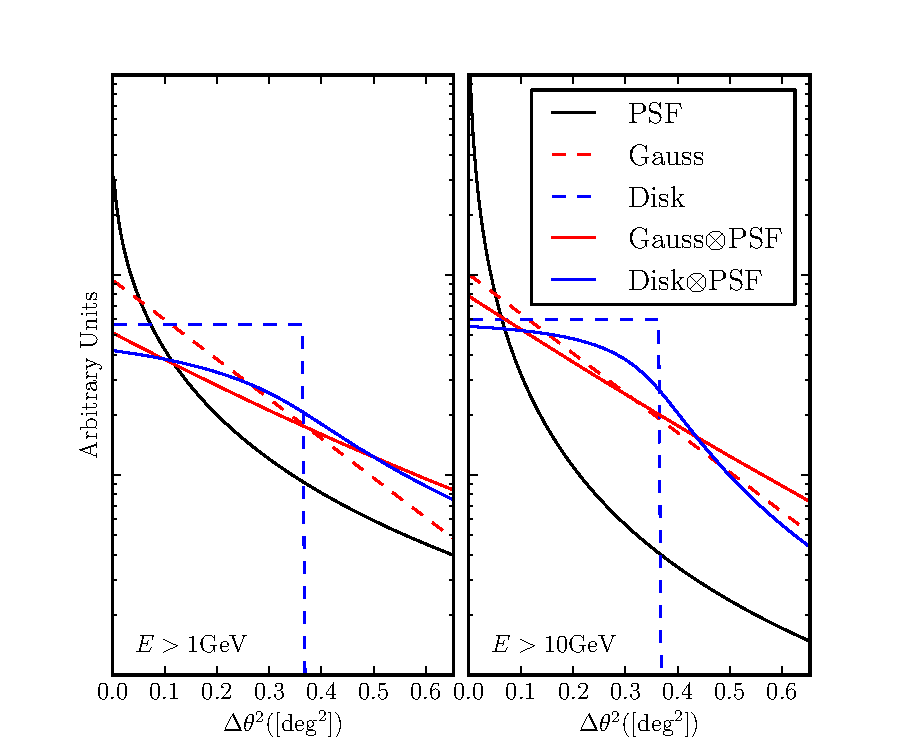
\includegraphics{mc_plots/compare_disk_gauss.pdf}
    % this plot came from /u/gl/lande/work/fermi/extended_catalog/2FGL/plots_for_paper/compare_disk_gauss/v2/compare_disk_gauss.pdf
    \end{center}
    \caption{
    This plot demonstrates that different spatial models when smoothed
    by the PSF look similar.  The $y$ axis is the log of the
    intensity and the $x$ axis is $\theta^2$.  The black line is the
    PSF that would be observed for a power-law source of spectral index
    2. The dashed red line is the probability density of a Gaussian with
    $\rsixeight=0.5\deg$, which is just a straight line on this plot
    The dashed blue line is the probability density for a uniform disk
    with $\rsixeight=0.5\deg$.  Finally, the solid red and blue lines
    show the convolution of the Gaussian and uniform disk with the PSF.
    The left plot shows the analysis with an energy range from 1 \gev to
    100 \gev whereas the right plot shows the analysis with an energy
    range from 10 \gev to 100 \gev.  This plot is discussed further in
    section~\ref{compare_source_size}.
    }\label{compare_disk_gauss}
  \end{figure}

  \begin{figure}
    \begin{center}
      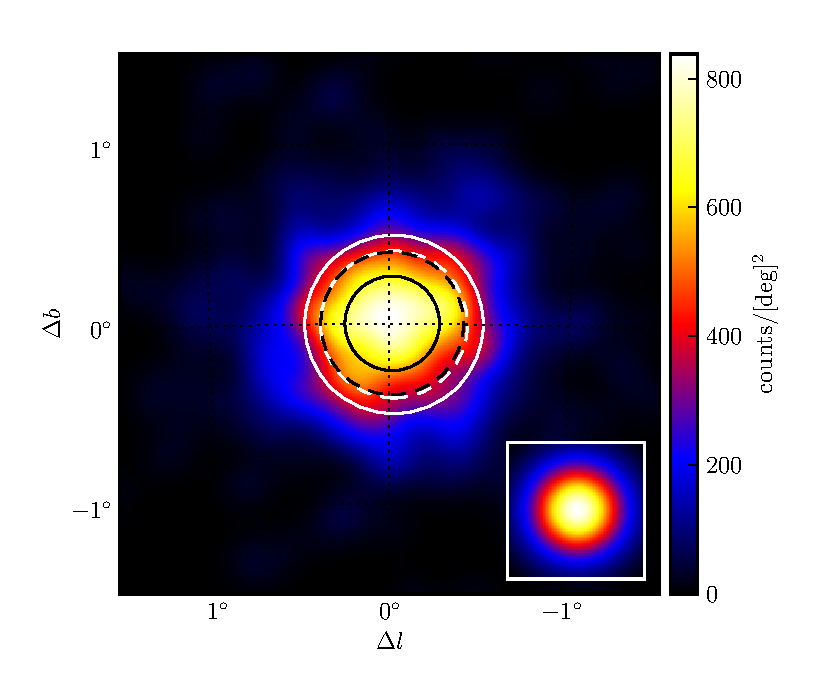
\includegraphics{mc_plots/compare_r68.pdf}
      % this plot came from /u/gl/lande/work/fermi/extended_catalog/2FGL/plots_for_paper/compare_r68/v2/plot.py
      \end{center}
      \caption{
      This plot shows that fitting the same source with different spatial
      shapes can lead to different values of $\sigma$. On the other
      hand, the different shapes have a good agreement about the 68\%
      containment radius \rsixeight.  It shows counts map for a simulated
      uniform disk extended source in the energy range from 1 \gev to
      100 \gev.  The source has a size $\sigma=0.5\deg$, an integral flux
      between 1 \gev and 100 \gev of $3\times 10^{-8}\ph/\cm^2/\sec$, and
      a spectral index 2.  The smoothed counts from a point source with
      the same spectrum are shown in the bottom right inset.  This source
      was fit with both a uniform disk and a Gaussian spatial model.
      The red circle represents the fit size $\sigma$ modeling the
      source with a uniform disk spatial model.  The black circle is
      the fit $\sigma$ modeling the source with a Gaussian hypothesis.
      The dashed white and black circle are the fit \rsixeight for the
      disk and Gaussian hypothesis. This plot is discussed further in
      section~\ref{compare_source_size}.
      }\label{compare_r68}
    \end{figure}


    \begin{table}
  \begin{centering}
    \begin{tabular}{ r | r | r | r }
      \hline
      \hline
      $\gamma$ & flux ($\ph/\cm^2/\sec$) & $N_\text{sims}$ & $\langle\ts\rangle$ \\
      \hline
      1.5 &          $10^{-6}$ &           31952 &  92862 \\
      &  $3\times 10^{-7}$ &           31962 &  22169 \\
      &          $10^{-7}$ &           31977 &   5806 \\
      &  $3\times 10^{-8}$ &           31991 &   1270 \\
      &          $10^{-8}$ &           31940 &    301 \\
      &  $3\times 10^{-9}$ &           30324 &     62 \\
      \hline
      2 &          $10^{-6}$ &           31872 &  22067 \\
      &  $3\times 10^{-7}$ &           31890 &   4898 \\
      &          $10^{-7}$ &           31858 &   1097 \\
      &  $3\times 10^{-8}$ &           31632 &    236 \\
      &          $10^{-8}$ &           27491 &    103 \\
      \hline
      2.5 &          $10^{-6}$ &           31822 &   4706 \\
      &  $3\times 10^{-7}$ &           31822 &    889 \\
      &          $10^{-7}$ &           31169 &    176 \\
      &  $3\times 10^{-8}$ &           21591 &     41 \\
      \hline                                                
      3 &          $10^{-6}$ &           31763 &    929 \\
      &  $3\times 10^{-7}$ &           31665 &    161 \\
      &          $10^{-7}$ &           19271 &     40 \\
      \hline
    \end{tabular}
    \caption{
    This table presents a list of the spectral models (flux and
    spectral index) used in the Monte Carlo study of \pointlike
    described in section~\ref{monte_carlo_validation} and presented
    in figure~\ref{ts_ext_mc}.  For each spectral model, the number of
    statistically independent simulations and the average value of \ts
    value ($\langle\ts\rangle$) is tabulated.  The Monte Carlo simulation
    spans parameters representative of sources that could be detected
    by the LAT.  The simulation is of spectral indices $\gamma$ of 1.5,
    2, 2.5, and 3.  The simulation is of fluxes varying from a $5\sigma$
    source detection to a $>10\sigma$ source detection.  Only simulations
    which produced statistically significant detections ($\ts>25$)
    were kept.  What is quoted is the $>100$ \mev integral flux measured
    in units of $\ph/\cm^2/\sec$.  More information about this Monte
    Carlo analysis is presented in section~\ref{monte_carlo_validation}.
    }\label{ts_ext_num_sims}
  \end{centering}
\end{table}

\clearpage

\clearpage
\begin{figure}
  \begin{center}
    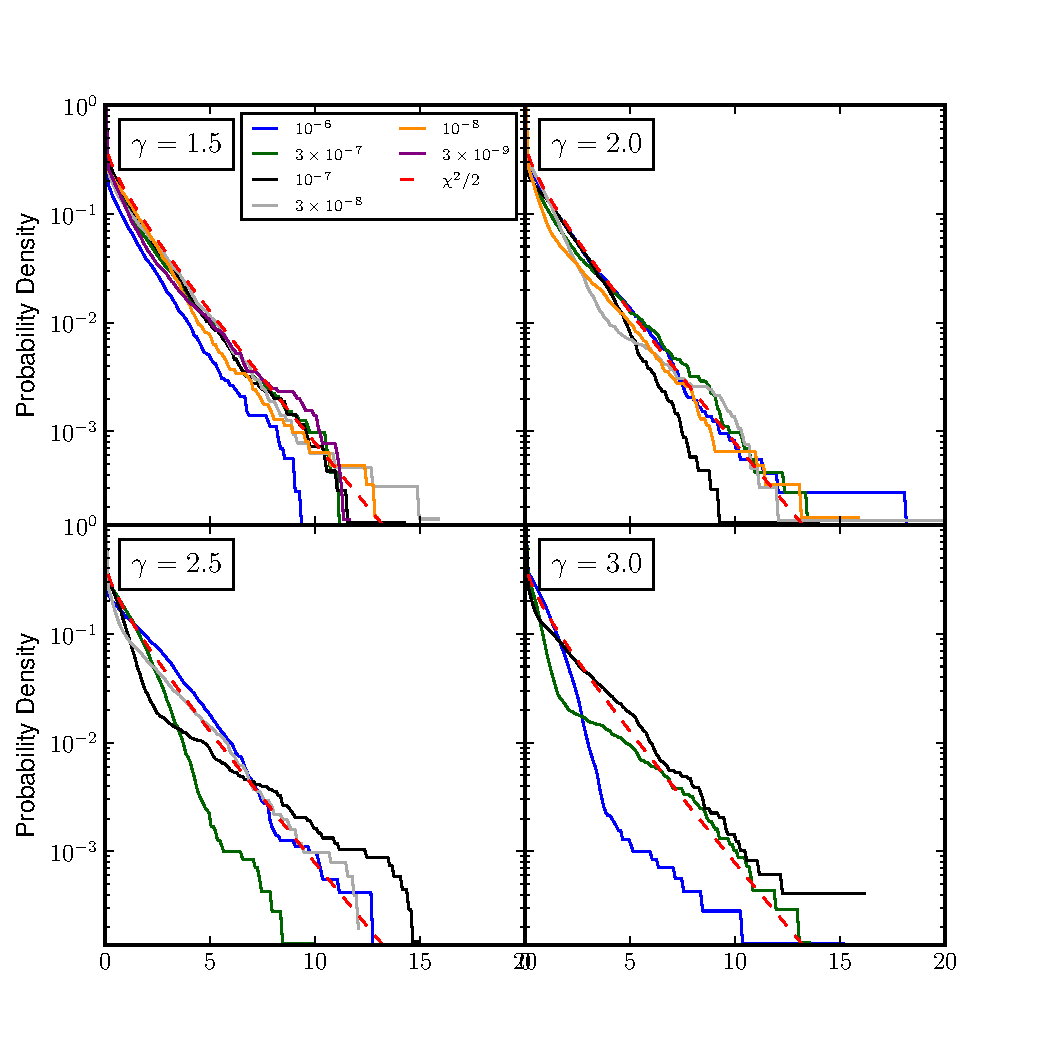
\includegraphics{mc_plots/ts_ext_emin_1000.pdf}
    % this plot came from /u/gl/lande/work/fermi/extended_catalog/monte_carlo/ts_ext/v3/plot.py
    % using data from /nfs/slac/g/ki/ki03/lande/extended_catalog/monte_carlo/ts_ext/v3_emin_1000/merged.hdf5
    \end{center}
    \caption{
    The results of the Monte Carlo simulation described
    in section \ref{monte_carlo_validation} and detailed in
    table~\ref{ts_ext_num_sims}. The plot shows the null distribution of
    the likelihood ratio test when fitting a point source for extension.
    The $x$ axis is \tsext and the $y$ axis is the cumulative density
    for \tsext of simulated point sources. The four plots represent
    different spectral indices and the different colors represent
    different fluxes.  The dashed red line is the cumulative density
    function of $\chi^2(\ts)/2$ which is suggested by Wilks' theorem
    as the distribution these curves should should follow.  There is
    a surprisingly good agreement between the Monte Carlo results and
    the theoretical distribution. For most spectral parameters, the
    Monte Carlo curve lies to the left of the theoretical curve which
    would make the theoretical distribution more conservative.  In this
    paper, we use this theoretical curve to estimate the significance of
    our source detections. This plot cuts off three simulations of the
    source with flux $3\times10^{-8}\ph/\cm^2/\sec$ and spectral index
    2.5 which had \tsext of 26.1, 28.9, and 38.1.
    }\label{ts_ext_mc}
  \end{figure}

\clearpage

\begin{figure}
  \begin{center}
    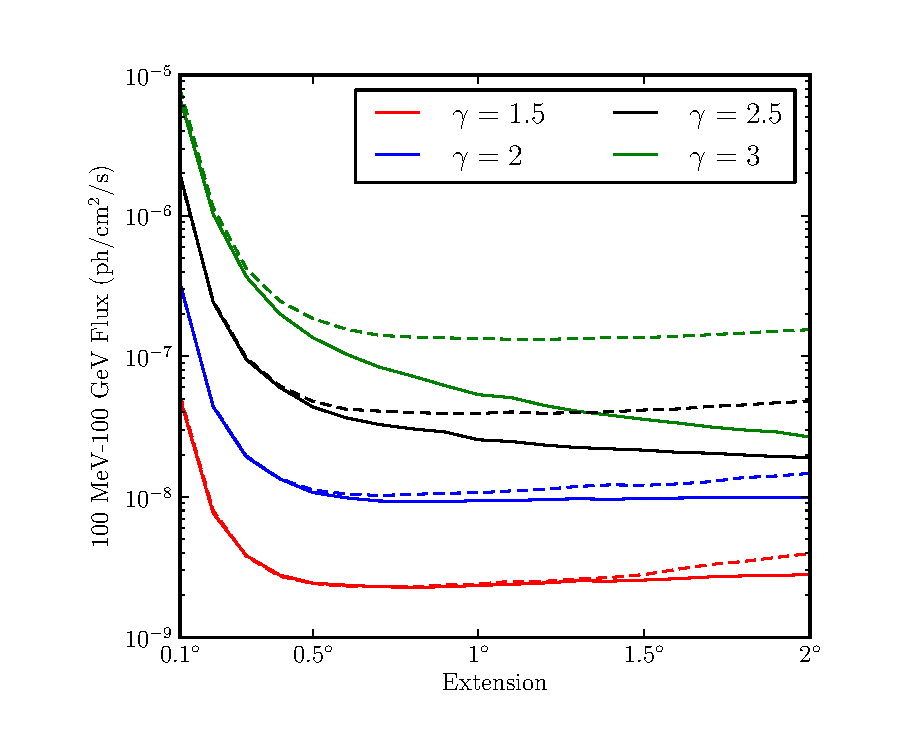
\includegraphics{mc_plots/index_sensitivity.pdf}
    % this plot came from /u/gl/lande/work/fermi/extended_catalog/monte_carlo/sensitivity/v9/plot_vs_index.py
    \end{center}
    \caption{
    This plot shows that our threshold to detecting the extension of
    a source is best for sources with size $~0.5\deg$. It also shows
    that for sources neither too large nor soft, our sensitivity is
    not significantly improved using photons with energy between 100
    \mev and 1 \gev.  The $x$ axis is extension of a simulated uniform
    disk extended source and the $y$ axis is the simulated source's 100
    \mev to 100 \gev photon flux. The curves represent the detection
    threshold to an extended source which is defined as the flux when
    $\langle\tsext\rangle=25$ for a particular extension.  All sources
    have an assumed power-law spectrum and the different colors are
    for sources of different simulated spectral indices.  The dashed
    line shows simulations using photons with energy between 100 \mev
    and 100 \gev while the solid lien shows simulations using photons
    with energy between 1 \gev and 100 \gev.  The detection threshold
    is for a one year simulation against a Sreekumar-like isotropic
    background.  More information about this plot is presented in
    section~\ref{extension_sensitivity}.
    }\label{index_sensitivity}
  \end{figure}

\clearpage

\begin{figure}
  \begin{center}
    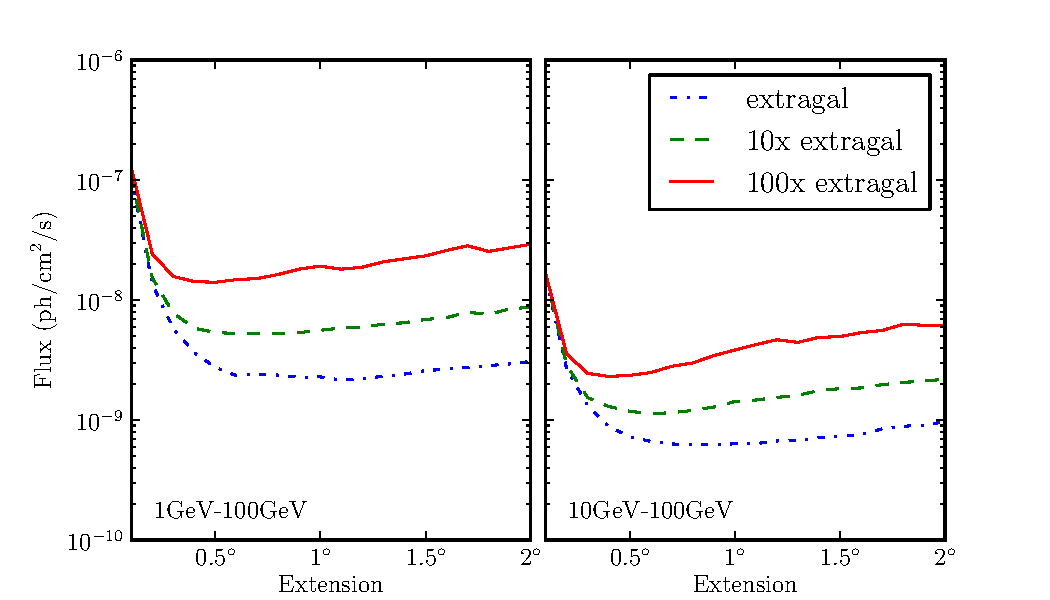
\includegraphics{mc_plots/diff_factor_sensitivity.pdf}
    % this plot came from /u/gl/lande/work/fermi/extended_catalog/monte_carlo/sensitivity/v9/plot_vs_diff_factor.py
    \end{center}
    \caption{
    This plot shows that we are less sensitive to extended sources in
    regions with higher background and (given the same number of photons)
    more sensitive to harder sources.  The plot has the same meaning as
    in figure~\ref{index_sensitivity} and the simulations occur over
    the same time range.  These plots presents the sensitivity over
    for varying background levels and two energy ranges.  The blue dash
    dotted plot is the sensitivity against a Sreekumar-like isotropic
    background. The green dashed curve shows the sensitivity against 10
    times that isotropic background and the solid red curve shows the
    sensitivity against 100 times that isotropic background.  The latter
    factor approximately represents the intensity of the galactic
    diffuse emission near the galactic center.  The left plot presents
    the sensitivity when using only photons with energies between 1 \gev
    and 100 \gev while the plot on the right presents the sensitivity only
    when using photons with energies between 10 \gev and 100 \gev. Unlike
    figure~\ref{index_sensitivity}, the sensitivity was calculated only
    for a power-law source of spectral index 2. Similarly, the flux is
    quoted only in the selected energy range which weakens the dependence
    of the detection threshold on spectral index.  More information
    about this plot is presented in section~\ref{extension_sensitivity}.
    }\label{diff_factor_sensitivity}
  \end{figure}


\begin{figure}
  \begin{center}
  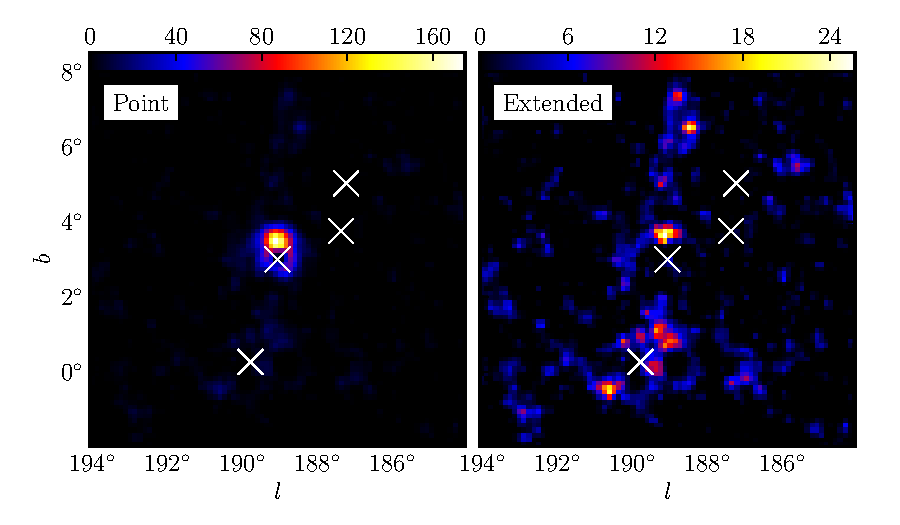
\includegraphics{ic443_plots/res_tsmap_ic443.pdf}
  % plot from /u/gl/lande/work/fermi/extended_catalog/2FGL/plots_for_paper/res_tsmap_ic443/v1

  \caption{An example residual test statistic map generated for the
  supernova remnant IC443 using photons with energy between 1 \gev and
  100 \gev.  The top plot is the residual TS map fitting IC443
  as a point source and the bottom plot is the residual TS map fitting
  IC443 as an extended source. The crosses in the plot represent all of
  the sources fit in the region. Since there is a residual TS greater
  than 160 fitting with the point hypothesis, it is clear that a point
  source is not a good fit to the region. On the other hand,
  the residual TS fitting as an extended source is much lower, showing
  that IC443 is better fit by an extended source. These plots were generated
  for all extended source candidates to help validate the analysis.}
  \label{res_tsmaps}
  \end{center}
\end{figure}

\clearpage
\begin{figure}
  \begin{center}
    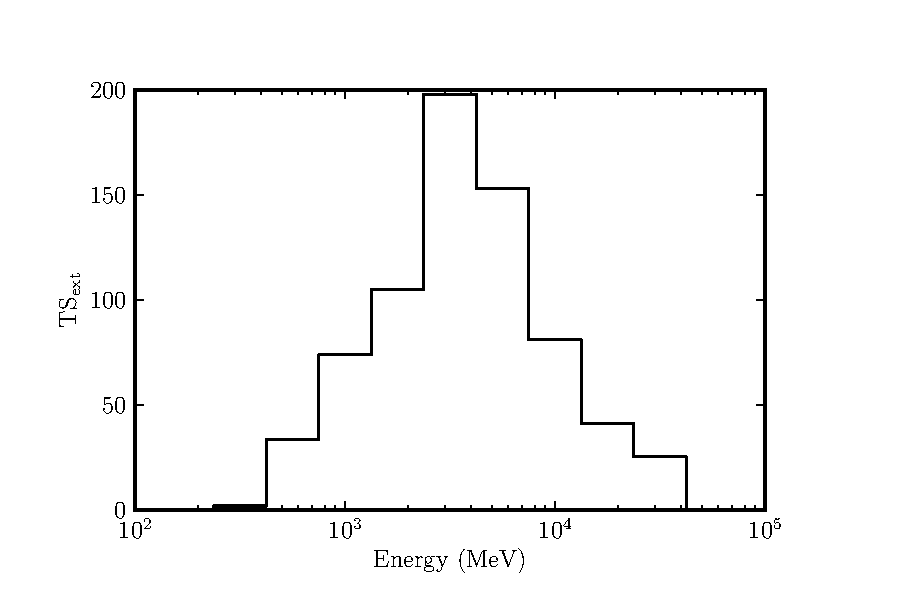
\includegraphics{ic443_plots/ic443_ts_ext_vs_energy.pdf}
    % taken from /u/gl/lande/work/fermi/extended_catalog/2FGL/plots_for_paper/ts_ext_vs_energy/v1/ts_ext_vs_energy.py
    \caption{
    The plot shows \tsext for 12 uniform log(energy) bins between 100 \mev
    and 100 \gev for the SNR IC443. IC443 has a spectral index $~2.4$
    (table~\ref{known_extended_sources}) which is typical of extended
    sources.  This plot shows that there is little gain in sensitivity to
    the extension of a source using photons with energies below 1 \gev.
    For this reason, this paper restricts its analysis to energies above
    1 \gev.
    }
    \label{ts_ext_vs_energy}
  \end{center}
\end{figure}

\clearpage
\begin{figure}
  \begin{center}
    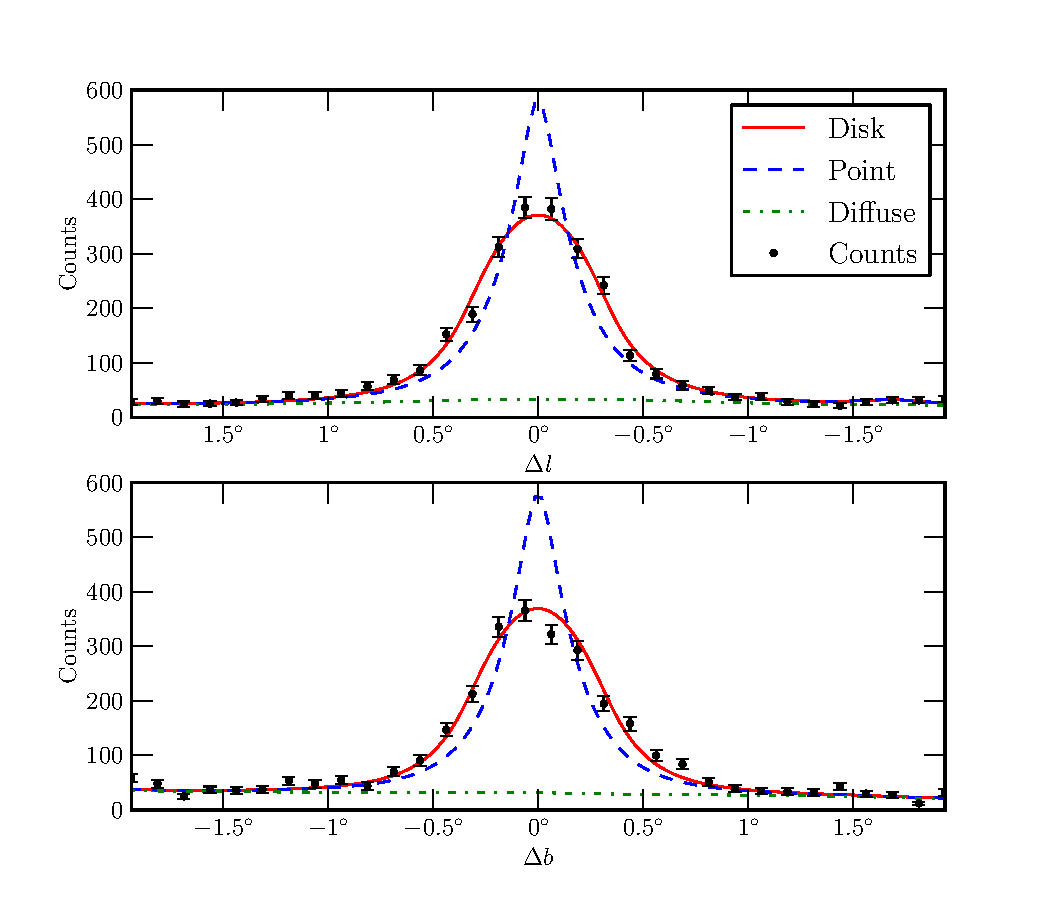
\includegraphics{ic443_plots/ic443_counts_slice.pdf}
    % taken from /u/gl/lande/work/fermi/extended_catalog/2FGL/plots_for_paper/counts_slice_ic443/v1/ic443_counts_slice.pdf
    \caption{ The upper plot is the sum of the counts binned in galactic
    longitudinal summed within 2\deg in galactic latitude centered on the
    SNR IC443. The lower plot shows the same image but instead integrated
    in galactic longitude.  Overlaid on the plot is the model predicted
    counts assuming that IC443 is a point source, an extended source, and
    that there is just the diffuse background.  These plots were generated
    for all extended source candidates.  They are especially useful for
    visually assessing the quality of the diffuse emission model in the
    region surrounding an extended source candidate.} \label{counts_slice}
  \end{center}
\end{figure}

\clearpage
\begin{figure}
  \begin{center}
    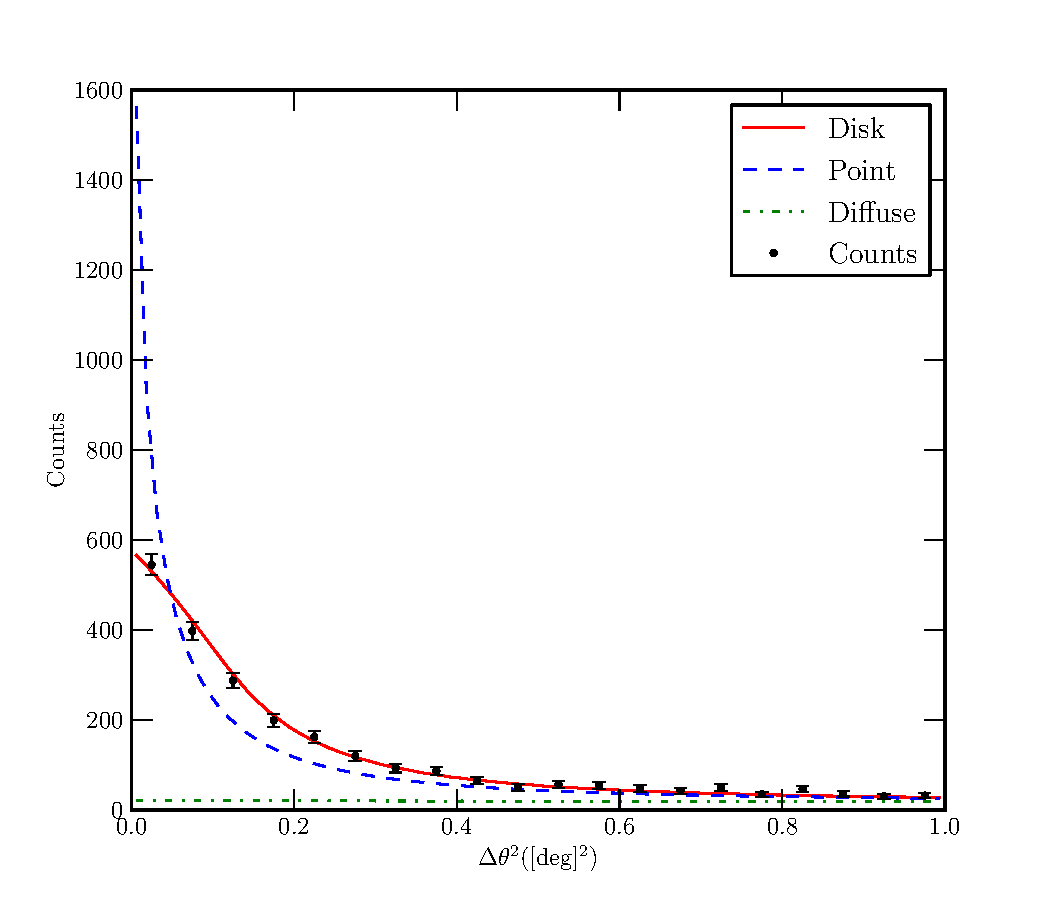
\includegraphics{ic443_plots/ic443_radial_integral.pdf}
    % taken from /u/gl/lande/work/fermi/extended_catalog/2FGL/plots_for_paper/radial_integral_ic443/v1/ic443_radial_integral.pdf
    \caption{The sum of all counts within a given radial distance from
    the SNR IC443's best fit position.  This plot is binned uniformly
    in $\theta^2$ to correct for solid angle so that an isotropic
    distribution is flat. Overlaid on the counts distribution is the
    model predicted counts assuming the IC4343 is a point source, an
    extended source, and that there is just the diffuse background.
    These plots were generated for all extended source candidates.
    These radial integral plots are useful for visually comparing the
    observed counts to the PSF.}
    \label{radial_profile}
  \end{center}
\end{figure}

\clearpage
\begin{figure}
  \begin{center}
    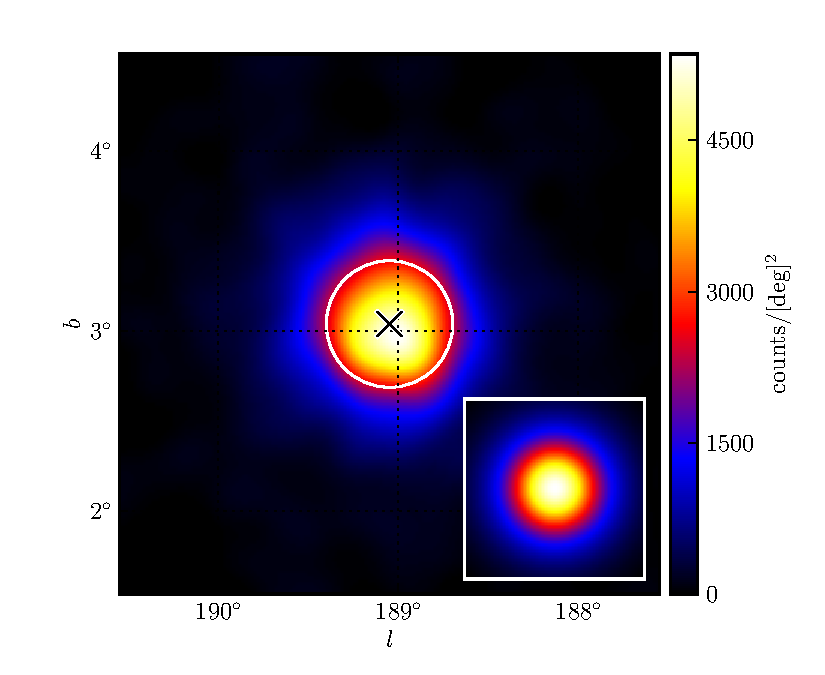
\includegraphics{ic443_plots/ic443_smoothed_counts.pdf}
    % taken from /u/gl/lande/work/fermi/extended_catalog/2FGL/plots_for_paper/smoothed_counts_ic443/v1
    \caption{A map of the observed photons in the region around the SNR
    IC443 with energies between 1 \gev and 100 \gev.  This plot has the
    galactic and isotropic diffuse emission subtracted and is smoothed
    by a $0.1\deg$ Gaussain kernel.  The overlaid box is the PSF for
    a source of the same spectrum as IC443 normalized to have the same
    intensity as IC443.  This PSF is smoothed by the same Gaussian kernel
    and so represents the model of what IC443 would look like if it was
    a point source. Since the observed counts are wider than the PSF,
    we can see visually that IC443 is an extended source.  The black
    cross is IC443's best fit center when fitting it with a uniform
    disk spatial model. The
    black crosses are all of the catalog sources in
    the region and the red circle is the edge of the best fit
    uniform disk which was fit to IC443 using \pointlike.  These plots
    were generated for all extended source candidates.  They are useful
    for assessing the overall quality of the source model and for looking
    for nearby background sources which are not correctly modeled.}
    \label{smoothed_counts}
  \end{center}
\end{figure}

\clearpage
\begin{figure}
  \begin{center}
    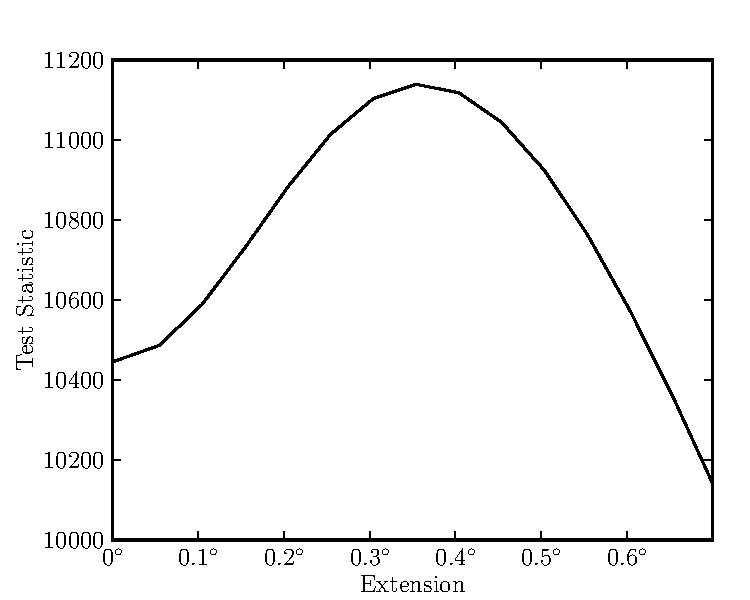
\includegraphics{ic443_plots/profile_ic443.pdf}
    % taken from /u/gl/lande/work/fermi/extended_catalog/2FGL/plots_for_paper/extension_profile_ic443/v1/profile_ic443.pdf
    \caption{
    A plot of the overall change in \ts when varying the
    extension of the extended SNR IC443.  As is discussed in section
    \ref{extension_error}, the error on the extension of a source is
    calculated by varying the extension away from its best fit value until
    the \loglikelihood has changed by a particular amount.  These profiles are
    generated for all extended source candidates. They are useful
    to make sure the fitter find a global minimum and that
    the likelihood function is not unphysically double peaked.
    }
    \label{extension_profile}
  \end{center}
\end{figure}


\clearpage
\begin{figure}
  \begin{center}
    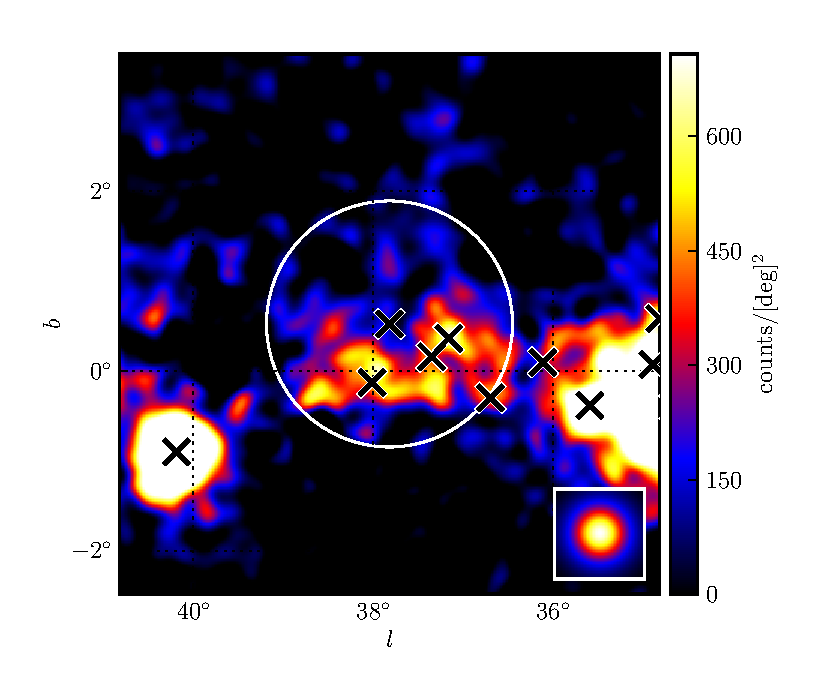
\includegraphics{source_plots/example_bad_fit.pdf}
    % taken from /u/gl/lande/work/fermi/extended_catalog/2FGL/plots_for_paper/example_bad_fit/v2
    \caption{
    The observed 1 \gev to 100 \gev photons for the
    two year catalog source 2FGL J1856.2+0450c. This map is smoothed by
    a 0.1\deg Gaussian kernel and the red circle is the edge of
    the fit uniform disk spatial model.  2FGL J1856.2+0450c fits to an
    extension of 1.37\deg and the result is statistically significant
    with \tsext=51.6. On the other hand, the extension encompasses many
    catalog sources and the emission does not look to be uniform. Instead,
    this source is fitting large scale residual. Although the fit is 
    statistically significant, it is not physical and we discard sources
    that look like this.
    }
    \label{example_bad_fit}
  \end{center}
\end{figure}


\clearpage
\begin{sidewaystable}
    \begin{centering}
      \begin{tabular}{l|rrrrrrrrrr}
        \hline
        \hline
        Name                 &          \glon &          \glat &                    $\sigma$ &         TS &   $\tsext$ &      Major &      Minor &        Ang &      Flux ($10^{-9}$) &                 Index \\
        \hline
        \multicolumn{11}{c}{$E > 1 \gev$} \\
        \hline
        SMC                  &     302.87\deg &     -44.65\deg & $  1.59\deg \pm   0.15\deg$ &       93.1 &       51.2 &  0.173\deg &  0.129\deg &   41.9\deg & $    3.0 \pm     0.4$ & $   2.42 \pm    0.16$ \\
        LMC                  &     278.58\deg &     -32.82\deg & $  2.26\deg \pm   0.09\deg$ &      384.2 &      304.4 &  0.096\deg &  0.071\deg &  -35.5\deg & $   12.9 \pm     0.7$ & $   2.42 \pm    0.08$ \\
        IC443                &     189.05\deg &       3.04\deg & $  0.35\deg \pm   0.01\deg$ &    10765.3 &      535.3 &  0.006\deg &  0.006\deg &   84.0\deg & $   65.2 \pm     1.2$ & $   2.23 \pm    0.02$ \\
        W28                  &       6.51\deg &      -0.29\deg & $  0.39\deg \pm   0.02\deg$ &     1231.3 &       92.1 &  0.014\deg &  0.013\deg &   30.4\deg & $   55.9 \pm     1.8$ & $   2.65 \pm    0.03$ \\
        W30                  &       8.61\deg &      -0.20\deg & $  0.36\deg \pm   0.04\deg$ &      458.1 &       66.0 &  0.020\deg &  0.018\deg &   14.1\deg & $   30.0 \pm     1.8$ & $   2.58 \pm    0.06$ \\
        W44                  &      34.68\deg &      -0.42\deg & $  0.34\deg \pm   0.02\deg$ &     1387.6 &      111.3 &  0.009\deg &  0.009\deg &  -39.4\deg & $   74.7 \pm     1.0$ & $   2.67 \pm    0.01$ \\
        W51C                 &      49.12\deg &      -0.44\deg & $  0.28\deg \pm   0.02\deg$ &     2174.7 &       87.6 &  0.010\deg &  0.010\deg &   59.4\deg & $   41.6 \pm     1.3$ & $   2.38 \pm    0.04$ \\
        Cygnus Loop          &      74.20\deg &      -8.51\deg & $  1.74\deg \pm   0.06\deg$ &      206.2 &      164.1 &  0.096\deg &  0.063\deg &  -69.0\deg & $    8.7 \pm     0.7$ & $   2.55 \pm    0.15$ \\
        \hline
        \multicolumn{11}{c}{$E > 10 \gev$} \\
        \hline
        MSH 15-52            &     320.39\deg &      -1.22\deg & $  0.20\deg \pm   0.06\deg$ &       73.7 &        9.5 &  0.033\deg &  0.032\deg &    3.9\deg & $    0.6 \pm     0.1$ & $   2.32 \pm    0.23$ \\
        HESS J1825-137       &      17.58\deg &      -0.46\deg & $  0.64\deg \pm   0.08\deg$ &       85.6 &       62.5 &  0.050\deg &  0.045\deg &   33.6\deg & $    1.8 \pm     0.3$ & $   1.75 \pm    0.20$ \\
      \end{tabular}
      \caption{The fit for ten of the twelve extended sources included
      in the second LAT catalog.  The top list are the extended sources
      analyzed using photons with energies between 1 \gev and 100 \gev.
      The lower table are the sources analyzed using photons with energies
      between 10 \gev and 100 \gev.  The quoted flux is in units of
      $10^{-9}\ph/\cm^2/\sec$ and is the flux in the fit energy range
      (either 1 \gev to 100 \gev or 10 \gev to 100 \gev).  All sources
      were fit using a uniform disk spatial template. The localization
      and extension were found using \pointlike while the TS and spectral
      values were calculated using \gtlike.  The TS value was computed
      assumgni the best fit uniform disk spatial model and \tsext
      compares the increase in \ts fitting the source with an extended
      spatial model to point model.  \glon and \glat are respectively
      the galactic longitude and galactic latitude of the source and
      $\sigma$ is the edge of the best fit uniform disk spatial model.
      The extended PWN Vela X is not include in this list because a phase
      cut would be required to remove the Vela pulsar (\cite{velax}).
      The extended Centaurus A lobes are not included because a radially
      symmetric uniform disk spatial model is a bad match to the observed
      emission (\cite{cen_a_lat}).  More information about these sources is
      in section~\ref{validate_known}.
      }
      \label{known_extended_sources}
    \end{centering}
\end{sidewaystable}

\clearpage
\begin{figure}
  \begin{center}
    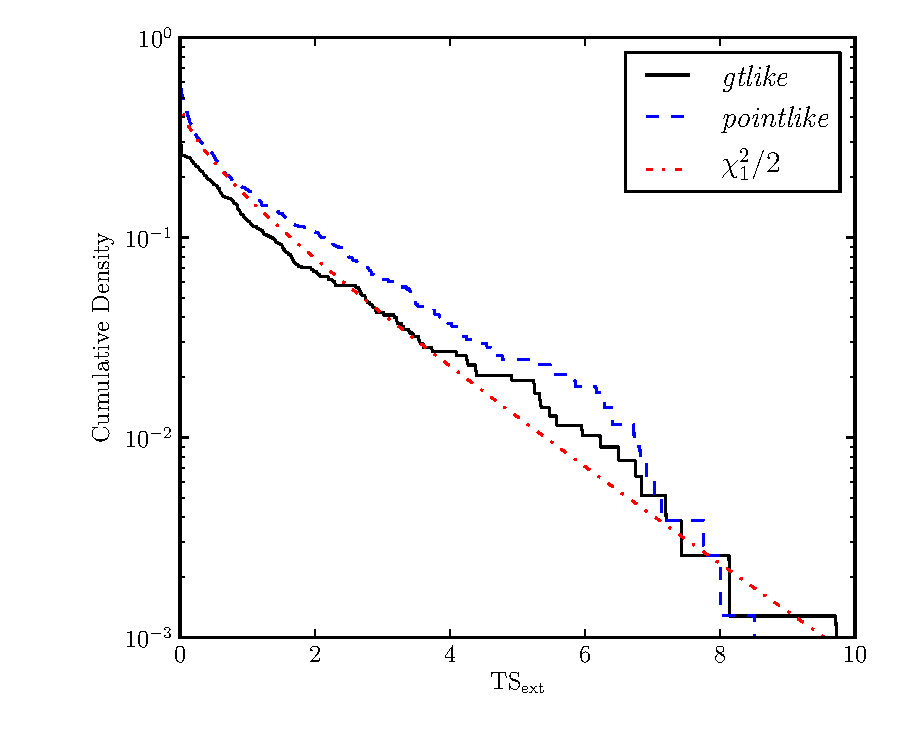
\includegraphics{source_plots/agn.pdf}
    % this plot came from /u/gl/lande/work/fermi/extended_catalog/2FGL/agn/v2/agn.py
    \end{center}
    \caption{The cumulative distribution of \tsext for 515 AGN associated
    in the first LAT AGN catalog using photons with energies between 1
    \gev and 100 \gev.  The method for selecting these AGN is described in
    section~\ref{test_1lac_sources}.  AGN are expected to be unresolvable
    so overlaid on this plot is a $\chi^2/2$ distribution suggested by
    Wilk's theorem.  The motivation for this distribution to hold is
    discussed in section~\ref{monte_carlo_validation}.  Overall, there
    is good agreement between this the fit values of \tsext and the
    $\chi^2/2$ distribution.  Possible reasons for the discrepancy between
    the distributions are discussed in section~\ref{test_1lac_sources}
    but this plot demonstrates that any systematics in our extension
    test are small compared to the signals we are looking for.
    }\label{agn_ts_ext}
  \end{figure}


  % 1FGL J1628.6-2419c - P72Y2516         - 2FGL J1627.0-2425c
  % 1FGL J1554.0-5345c - P72Y2405         - 2FGL J1554.4-5317c
  % 1FGL J0823.3-4248  - P72Y1212         - 2FGL J0823.0-4246
  % 1FGL J1614.7-5138c - P72Y2473         - 2FGL J1615.2-5138
  % 1FGL J1632.9-4802c - P72Y2540         - 2FGL J1632.4-4753c
  % 1FGL J2020.0+4049  - P72Y3281         - 2FGL J2021.5+4026
  % 1FGL J1837.5-0659c - P72Y2974         - 2FGL J1837.3-0700c
  % N/A                - P72Y1287         - 2FGL J0851.7-4635


\clearpage
\begin{sidewaystable}
  \begin{centering}
    \begin{tabular}{l|rrrrrrrrrr}
      \hline
      \hline
      Name                 &          \glon &          \glat &                    $\sigma$ &         TS &   $\tsext$ &      Major &      Minor &        Ang &      Flux ($10^{-9}$) &                 Index \\
      \hline
      \multicolumn{11}{c}{$E > 1 \gev$} \\
      \hline
      2FGL J0823.0-4246    &     260.32\deg &      -3.28\deg & $  0.37\deg \pm   0.03\deg$ &      314.7 &       46.1 &  0.026\deg &  0.023\deg &    5.3\deg & $    8.3 \pm     0.6$ & $   2.18 \pm    0.07$ \\
      2FGL J1627.0-2425c   &     352.87\deg &      16.79\deg & $  0.53\deg \pm   0.06\deg$ &      130.3 &       20.3 &  0.060\deg &  0.047\deg &   39.8\deg & $    6.7 \pm     0.7$ & $   2.48 \pm    0.15$ \\
      2FGL J1554.4-5317c   &     328.12\deg &       0.26\deg & $  0.52\deg \pm   0.04\deg$ &      150.8 &       37.6 &  0.044\deg &  0.039\deg &   55.5\deg & $   16.7 \pm     1.5$ & $   2.30 \pm    0.11$ \\
      2FGL J1712.4-3941    &     347.25\deg &      -0.54\deg & $  0.56\deg \pm   0.04\deg$ &       77.6 &       41.2 &  0.055\deg &  0.043\deg &  -14.8\deg & $    4.3 \pm     0.9$ & $   1.48 \pm    0.12$ \\
      \hline
      \multicolumn{11}{c}{$E > 10 \gev$} \\
      \hline
      2FGL J0851.7-4635    &     266.29\deg &      -1.41\deg & $  1.12\deg \pm   0.07\deg$ &      120.0 &       76.7 &  0.090\deg &  0.064\deg &   63.8\deg & $    1.3 \pm     0.1$ & $   1.75 \pm    0.08$ \\
      2FGL J1615.0-5051    &     332.38\deg &      -0.14\deg & $  0.33\deg \pm   0.04\deg$ &       54.0 &       16.6 &  0.049\deg &  0.040\deg &    1.7\deg & $    1.1 \pm     0.2$ & $   2.25 \pm    0.28$ \\
      2FGL J1615.2-5138    &     331.66\deg &      -0.66\deg & $  0.42\deg \pm   0.03\deg$ &       75.9 &       47.6 &  0.048\deg &  0.044\deg &   31.1\deg & $    1.1 \pm     0.2$ & $   1.77 \pm    0.26$ \\
      2FGL J1632.4-4753c   &     336.41\deg &       0.22\deg & $  0.44\deg \pm   0.04\deg$ &      128.3 &       64.8 &  0.042\deg &  0.036\deg &  -16.1\deg & $    2.0 \pm     0.2$ & $   2.29 \pm    0.22$ \\
      2FGL J1837.3-0700c   &      25.08\deg &       0.13\deg & $  0.35\deg \pm   0.08\deg$ &       47.0 &       20.2 &  0.075\deg &  0.064\deg &  -12.4\deg & $    1.1 \pm     0.2$ & $   1.65 \pm    0.21$ \\
      2FGL J2021.5+4026    &      78.17\deg &       2.19\deg & $  0.59\deg \pm   0.03\deg$ &      225.3 &      139.4 &  0.044\deg &  0.030\deg &   51.1\deg & $    1.8 \pm     0.2$ & $   2.31 \pm    0.19$ \\
      \hline
    \end{tabular}
    \caption{The 8 new source candidates found by the extended source
    search. Three new extended sources were found using photons with
    energies above 1 \gev and five new candidates were found using photons
    with energies above 10 \gev.  The columns in this table have the same
    meaning as in table~\ref{known_extended_sources}.  More information
    about these sources can be found in section~\ref{new_ext_srcs_section}.
    }
    \label{new_ext_srcs_table}
  \end{centering}
\end{sidewaystable}



\clearpage
\begin{sidewaysfigure}
  \begin{center}
    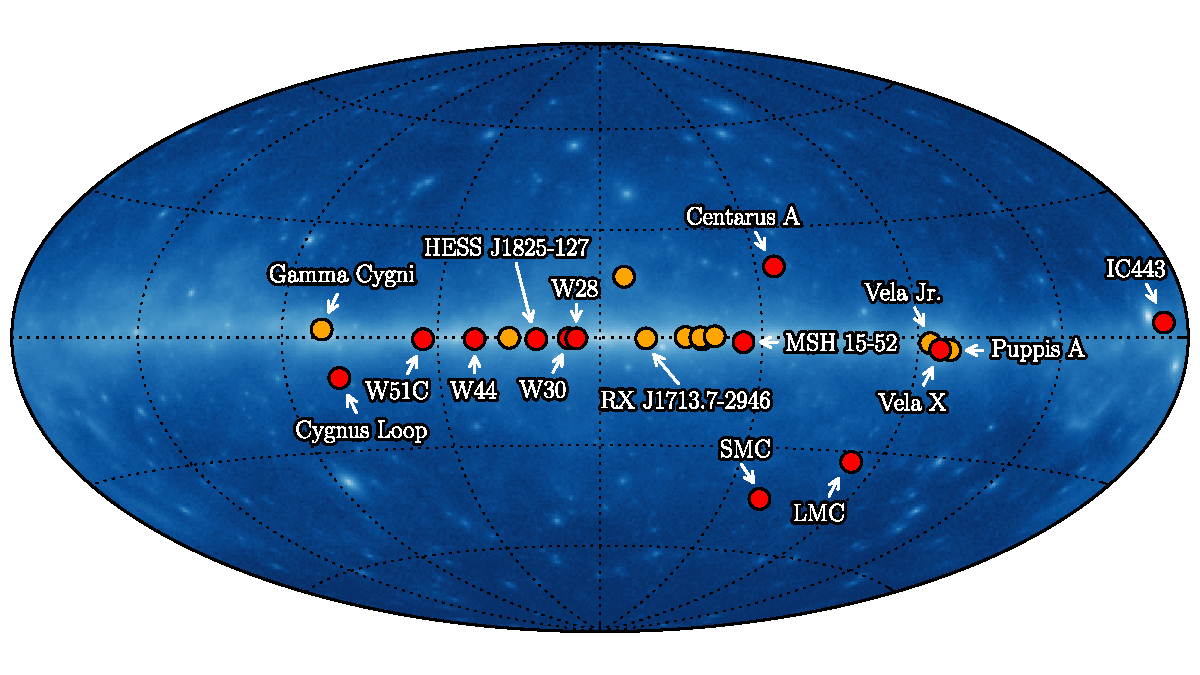
\includegraphics{summary_plots/allsky_extended_sources.pdf}
    % this plot came from /u/gl/lande/work/fermi/extended_catalog/2FGL/plots_for_paper/allsky/v1/run.py
    \end{center}
    \caption{A plot of all \gev extended sources detected by the LAT
    with two years of data.  The twelve extended sources included in
    the second LAT catalog are the red markers and the ten additional
    extended sources analyzed in this paper are the green markers. The
    extended sources are overlaid on an Aitoff projection Galactic
    coordinate map of all 100 \mev to 100 \gev photons measured by the
    LAT in the two year time interval of this analysis.}\label{allsky_extended_sources}
  \end{sidewaysfigure}

\clearpage
\begin{figure}
  \begin{center}
    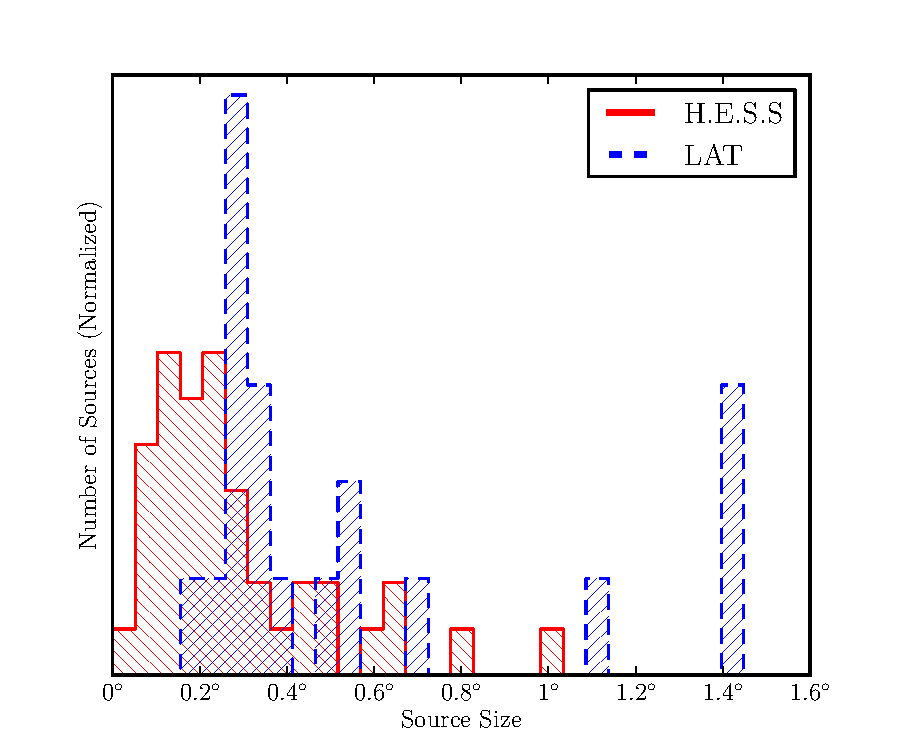
\includegraphics{summary_plots/gev_vs_tev_histogram.pdf}
    % this plot came from /u/gl/lande/work/fermi/extended_catalog/2FGL/plots_for_paper/extension_histogram/v1/extension_histogram.py
    \end{center}
    \caption{
    A comparison of the size of detected \tev and \gev sources.
    The extension of the 22 extended LAT sources comes from
    table~\ref{known_extended_sources}, table~\ref{new_ext_srcs_table},
    and the LAT extension of Vela X is taken from (\cite{velax}). The
    Centarus A lobes, which have an extension $~10\deg$, are not
    included in the plot (\cite{cen_a_lat}).  The \tev extension of
    the 42 extended H.E.S.S. sources comes from the H.E.S.S. Source
    Catalog (\cite{hesscat}).  Because the \gev sources were fit
    with a uniform disk spatial model whereas the \tev sources were
    fit with a Gaussian spatial model, the histogram is of \rsixeight
    (see section~\ref{compare_source_size}).  On the other hand, because
    of their size, the \tev size of RX J1713.7-2946 and Vela Jr. were
    obtained by a fit of a Gaussian spatial model so the \gev and \tev
    sizes of these sources were not converted.
    }\label{gev_vs_tev_histogram}
  \end{figure}

\clearpage
\begin{figure}
  \begin{center}
    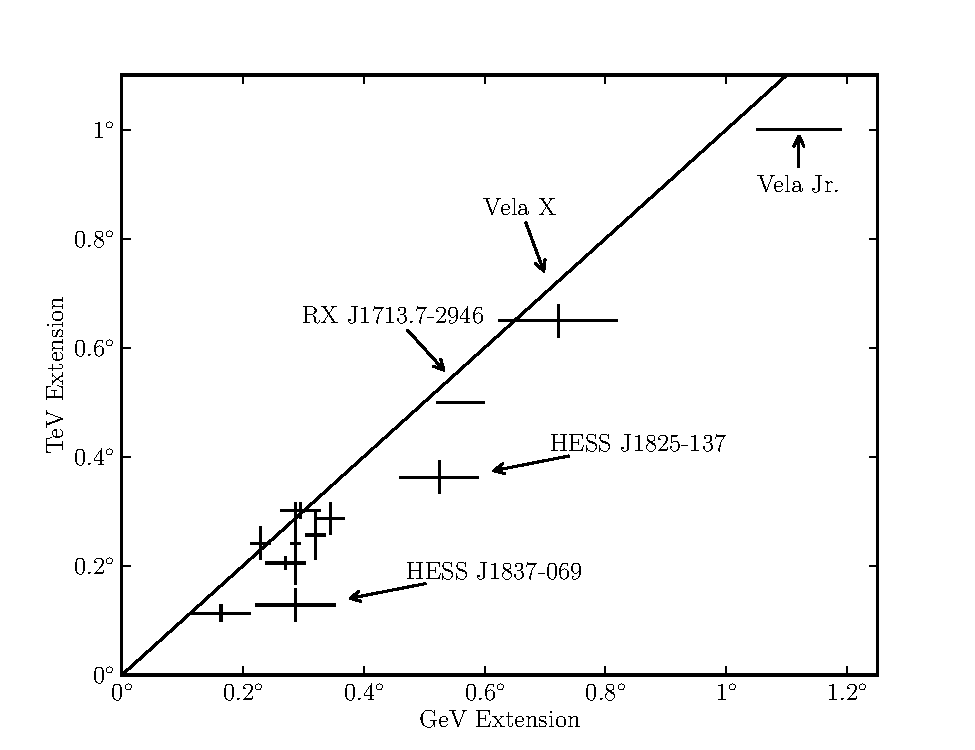
\includegraphics{summary_plots/gev_vs_tev_plot.pdf}
    % this plot came from /u/gl/lande/work/fermi/extended_catalog/2FGL/plots_for_paper/compare_tev_gev_sizes/v1/run.py
    \end{center}
    \caption{
    }\label{gev_vs_tev_plot}
  \end{figure}

\clearpage
\begin{sidewaystable}
    \begin{centering}
      \begin{tabular}{l|rr|rrrr|rrrr}
        \hline
        \hline
        Name                 &     \tsinc &     \tsext &      $\glon_1$ &      $\glat_1$ &   $\text{Flux}_1$ &   $\text{Index}_1$ &      $\glon_2$ &      $\glat_2$ &   $\text{Flux}_2$ &  $\text{Index}_2$ \\
        \hline
        \multicolumn{11}{c}{$E > 1 \gev$} \\
        \hline
        2FGL J0823.0-4246    &       21.9 &       46.1 &     260.59\deg &      -3.27\deg & $       2.0 \pm        0.5$ & $  1.9 \pm   0.2$  &     260.24\deg &      -3.20\deg & $       5.3 \pm        0.6$ & $  2.4 \pm   0.1$ \\
        2FGL J1627.0-2425c   &       19.1 &       20.3 &     353.00\deg &      16.97\deg & $       3.0 \pm        0.6$ & $  2.6 \pm   0.4$  &     353.26\deg &      16.67\deg & $       2.4 \pm        0.6$ & $  2.5 \pm   0.5$ \\
        2FGL J1554.4-5317c   &        9.2 &       37.6 &     328.30\deg &       0.31\deg & $      10.3 \pm        1.2$ & $  2.7 \pm   0.5$  &     328.27\deg &      -0.07\deg & $       0.9 \pm        0.6$ & $  1.6 \pm   0.4$ \\
        2FGL J1712.4-3941    &        6.6 &       41.2 &     347.28\deg &      -0.07\deg & $       0.2 \pm        0.1$ & $  0.6 \pm   0.5$  &     347.22\deg &      -0.26\deg & $       2.5 \pm        0.7$ & $  1.9 \pm   0.2$ \\
        \hline
        \multicolumn{11}{c}{$E > 10 \gev$} \\
        \hline
        2FGL J0851.7-4635    &       16.1 &       76.7 &     266.79\deg &      -1.32\deg & $       0.2 \pm        0.1$ & $  1.8 \pm   0.5$  &     266.41\deg &      -1.38\deg & $       0.2 \pm        0.1$ & $  1.5 \pm   0.6$ \\
        2FGL J1615.0-5051    &       12.2 &       16.6 &     332.39\deg &      -0.07\deg & $       0.4 \pm        0.1$ & $  2.3 \pm   0.6$  &     332.43\deg &      -0.36\deg & $       0.4 \pm        0.1$ & $  2.4 \pm   0.5$ \\
        2FGL J1615.2-5138    &       37.6 &       47.6 &     331.75\deg &      -0.37\deg & $       0.4 \pm        0.1$ & $  1.3 \pm   0.5$  &     331.46\deg &      -0.79\deg & $       0.4 \pm        0.1$ & $  2.0 \pm   0.5$ \\
        2FGL J1632.4-4753c   &       40.9 &       64.8 &     336.52\deg &       0.18\deg & $       0.7 \pm        0.2$ & $  2.8 \pm   0.5$  &     336.13\deg &       0.37\deg & $       0.5 \pm        0.1$ & $  1.7 \pm   0.4$ \\
        2FGL J1837.3-0700c   &       12.3 &       20.2 &      25.04\deg &       0.26\deg & $       0.3 \pm        0.1$ & $  1.2 \pm   0.6$  &      25.10\deg &      -0.05\deg & $       0.4 \pm        0.1$ & $  2.0 \pm   0.6$ \\
        2FGL J2021.5+4026    &       29.7 &      139.4 &      78.08\deg &       2.53\deg & $       0.4 \pm        0.1$ & $  2.0 \pm   0.5$  &      78.43\deg &       2.55\deg & $       0.5 \pm        0.1$ & $  1.8 \pm   0.4$ \\
        \hline
      \end{tabular}
      \label{dual_localization_results}
      \caption{For the new extended source candidates
      in table~\ref{new_ext_srcs_table}, we describe the
      results of the dual localization procedure described in
      section~\ref{dual_localization_method}. Here, the extended
      source candidate is not fit as an extended source but instead
      fit as two point sources.  The dual localization is performed
      with \pointlike and results in the best fit position of the two
      sources $(\glon_1,\glat_1)$ and $(\glon_2,\glat_2)$.  The change
      in likelihood and spectral values are then computed using \gtlike
      with the best fit positions found by \pointlike.  \tsinc is the
      increase in TS fitting the region as two sources compared to
      fitting compared to fitting a single point source and is computed
      using \gtlike with the best fit positions taken from \pointlike.
      It can be directly compared to \tsext, which is taken from
      table~\ref{new_ext_srcs_table}.  For all of our candidates, $\tsext
      > \tsinc$ which shows that an extended source fits the source better
      than two point sources.  As in table~\ref{known_extended_sources},
      flux is measured in units of $10^{-9}\ph/\cm^2/\sec$ and is the
      integral flux between 1 \gev (10 \gev) and 100 \gev for the sources
      found using photons above 1 \gev (10 \gev).}
    \end{centering}
  \end{sidewaystable}


  \clearpage
  \begin{sidewaystable}
    \begin{centering}
      \begin{tabular}{l|rrrrrrrr}
        \hline
        \hline
        Name                 &     $\ts_\pointlike$ &        $\ts_\gtlike$ &           $\ts_\alt$ &          \tsextpointlike &           \tsextgtlike &            \tsextalt &                    $\sigma$ &               $\sigma_\alt$ \\
        \hline
        \multicolumn{9}{c}{$E > 1 \gev$} \\
        \hline
        2FGL J0823.0-4246    &                347.3 &                314.7 &                343.9 &                     66.1 &                   46.1 &                 53.4 & $  0.37\deg \pm   0.03\deg$ & $  0.40\deg \pm   0.03\deg$ \\
        2FGL J1627.0-2425c   &                154.9 &                130.3 &                102.4 &                     32.6 &                   20.3 &                 23.8 & $  0.53\deg \pm   0.06\deg$ & $  0.39\deg \pm   0.04\deg$ \\
        2FGL J1554.4-5317c   &                134.8 &                150.8 &                139.4 &                     39.4 &                   37.6 &                 38.0 & $  0.52\deg \pm   0.04\deg$ & $  0.55\deg \pm   0.04\deg$ \\
        \hline
        \multicolumn{9}{c}{$E > 10 \gev$} \\
        \hline
        2FGL J0851.7-4635    &                120.2 &                120.0 &                126.1 &                     90.1 &                   76.7 &                 82.9 & $  1.12\deg \pm   0.07\deg$ & $  1.12\deg \pm   0.08\deg$ \\
        2FGL J1615.0-5051    &                 52.5 &                 54.0 &                 57.4 &                     17.5 &                   16.6 &                 12.4 & $  0.33\deg \pm   0.04\deg$ & $  0.33\deg \pm   0.04\deg$ \\
        2FGL J1615.2-5138    &                 76.2 &                 75.9 &                 89.4 &                     44.3 &                   47.6 &                 55.9 & $  0.42\deg \pm   0.03\deg$ & $  0.43\deg \pm   0.03\deg$ \\
        2FGL J1632.4-4753c   &                126.9 &                128.3 &                120.4 &                     64.0 &                   64.8 &                 63.7 & $  0.44\deg \pm   0.04\deg$ & $  0.44\deg \pm   0.04\deg$ \\
        2FGL J1837.3-0700c   &                 45.5 &                 47.0 &                 39.0 &                     18.6 &                   20.2 &                 16.6 & $  0.35\deg \pm   0.08\deg$ & $  0.35\deg \pm   0.07\deg$ \\
        2FGL J2021.5+4026    &                236.5 &                225.3 &                240.5 &                    156.0 &                  139.4 &                148.8 & $  0.59\deg \pm   0.03\deg$ & $  0.60\deg \pm   0.03\deg$ \\
      \end{tabular}
      \label{alt_diff_model_results}
      \caption{
      This table shows a comparison of the \ts values gotten using \gtlike
      and \pointlike.  It also compares the fit values using the standard
      diffuse model and using the alternate diffuse model described
      in section~\ref{alt_diff_model_description}.  $\ts_\pointlike$
      is the \ts of the source fit with the extended hypothesis using
      \pointlike whereas $\ts_\gtlike$ is the same quantity using the
      same model but fitting with \gtlike.  There is good agreement
      between the two methods.
      }
    \end{centering}
  \end{sidewaystable}

\begin{figure}
  \begin{center}
    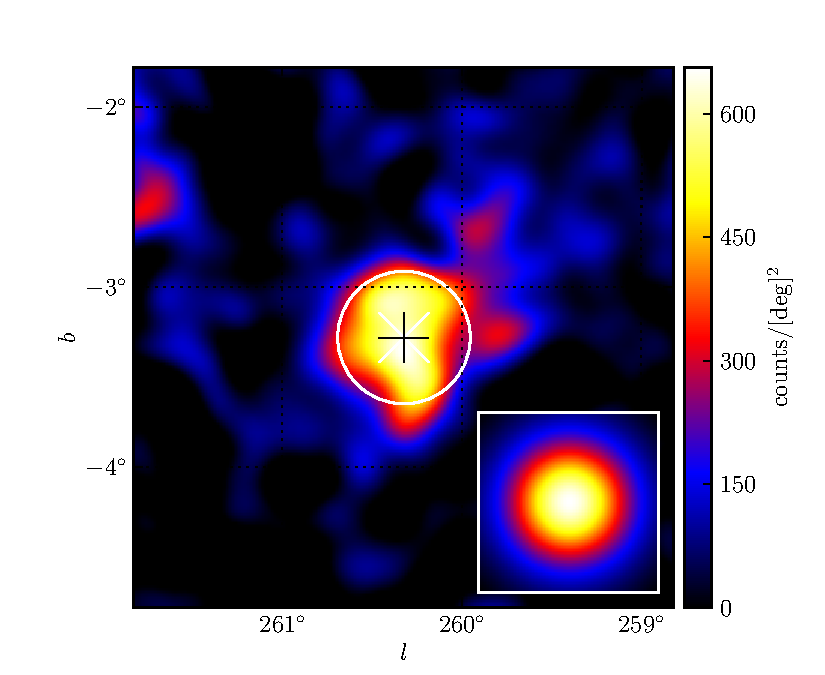
\includegraphics[type=pdf,ext=.pdf,read=.pdf]{source_plots/source_1FGL_J0823.3-4248}
  \end{center}
  % this plot came from 
  % /u/gl/lande/work/fermi/extended_catalog/2FGL/plots_for_paper/source_plots/1FGL_J0823.3-4248/v2/source_1FGL_J0823.3-4248.pdf
  \caption{A galactic and isotropic diffuse subtracted 1 \gev to 100
  \gev counts map of the region around 2FGL J0823.0-4246 smoothed by a
  0.1\deg Gaussian kernel.  The red star is the catalog position of this source.  
  The red cross and circle are the best fit position
  and extension of this source assuming a uniform disk spatial model.
  The two green stars are the positions of the sources 2FGL J0823.4-4305
  and 2FGL J0821.0-4254 which were removed because they are part of the
  extended source.  This source is spatially coincident with the Puppis
  A SNR. The light blue contours are an X-ray image of Puppis A observed by
  ROSAT (\cite{rosat_puppis_a}). There is good spatial overlap between
  the LAT and X-ray emission.  Even though the Vela pulsar is over 3
  degrees away from the source, because it is so bright it can be seen
  on the top left.  More information about this source can be found in 
  section~\ref{section_2FGL_J0823.0-4246}.
  }\label{1FGL_J0823.3-4248}
\end{figure}

\begin{figure}
  \begin{center}
    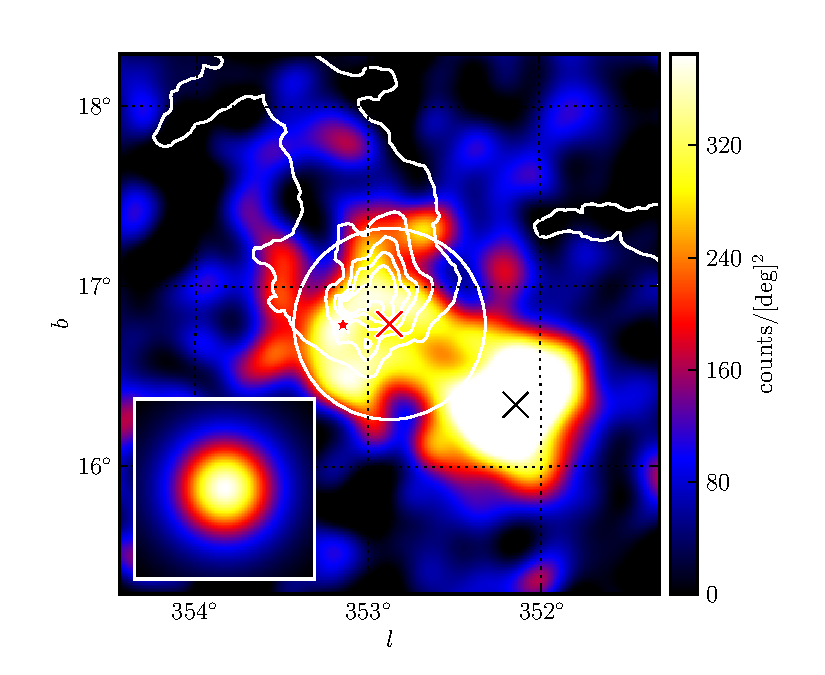
\includegraphics[type=pdf,ext=.pdf,read=.pdf]{source_plots/source_1FGL_J1628.6-2419c}
  \end{center}
  % this plot came from 
  % /u/gl/lande/work/fermi/extended_catalog/2FGL/plots_for_paper/source_plots/1FGL_J1628.6-2419c/v2/run.py
  \caption{
  A galactic and isotropic diffuse subtracted 1 \gev to 100 \gev counts
  map of the region around 2FGL J1627.0-2425 smoothed by a 0.1\deg
  Gaussian kernel.  The red star is the catalog's position of
  this source.  The red cross and circle are
  the best position and extension of this source assuming a
  uniform disk spatial model.  The black cross is the background source
  2FGL J1625.7-2526.  The light blue contours are a 100 micrometer infrared
  image of the region as seen by IRAS (\cite{iras_rho_ophiuci}). This
  source is in the Ophiuchus region and most likely represents 
  unmodeled diffuse emission.  More information about this source can be found
  in section~\ref{section_2FGL_J1627.0-2425c}.
  }\label{1FGL_J1628.6-2419c}
\end{figure}

\begin{figure}
  \begin{center}
    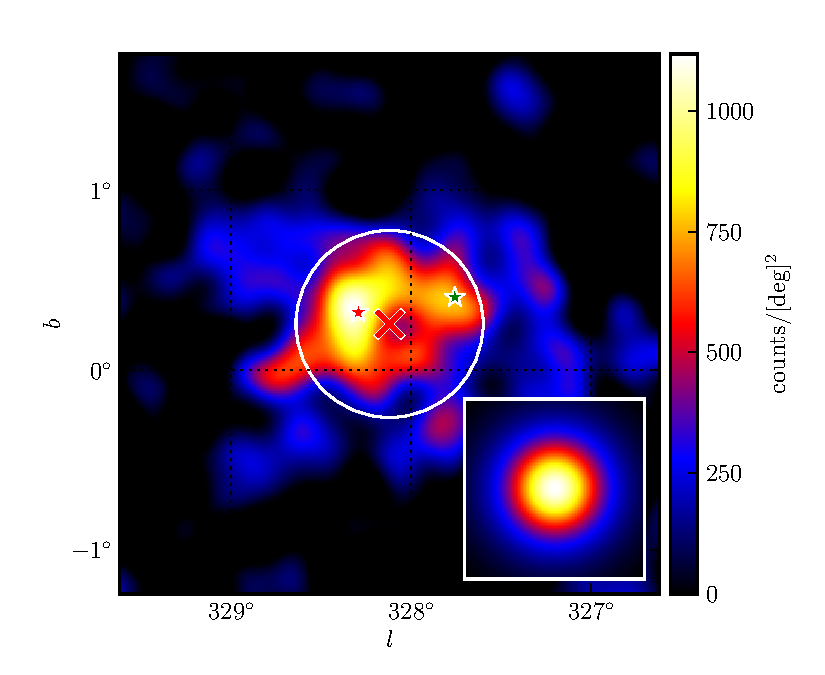
\includegraphics[type=pdf,ext=.pdf,read=.pdf]{source_plots/source_1FGL_J1554.0-5345c}
  \end{center}
  % this plot came from 
  % /u/gl/lande/work/fermi/extended_catalog/2FGL/plots_for_paper/source_plots/1FGL_J1554.0-5345c/v2/source_1FGL_J1554.0-5345c.pdf
  \caption{
  A galactic and isotropic diffuse subtracted 1 \gev to 100 \gev
  counts map of the region around 2FGL J1554.4-5317c smoothed by a
  0.1\deg Gaussian kernel.  The red star is the catalog position of
  2FGL J1554.4-5317c.  The red cross and circle are the best
  fit position and extension of this source assuming a uniform disk
  spatial model.  The green star represents the catalog source 2FGL
  J1551.3-5333c which was removed because it was part of
  the extended source.  Because the source has no obvious counterpart and
  is in a region of large diffuse emission, the source is most likely
  unmodeled diffuse emission.  More information about this source can be
  found in section~\ref{section_2FGL_J1554.4-5317c}.
  }
  \label{1FGL_J1554.0-5345c}
\end{figure}

\begin{figure}
  \begin{center}
    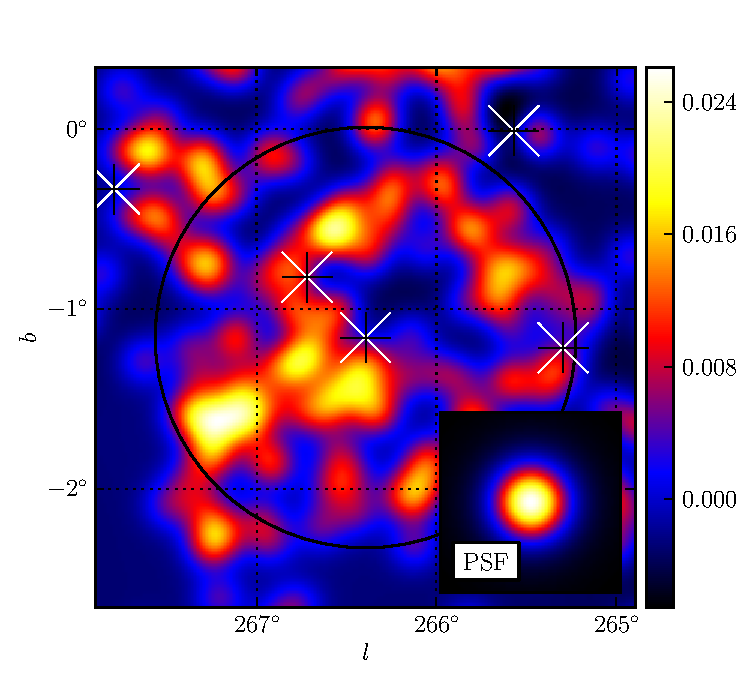
\includegraphics[type=pdf,ext=.pdf,read=.pdf]{source_plots/source_Vela_Jr}
  \end{center}
  % this plot came from 
  % /u/gl/lande/work/fermi/extended_catalog/2FGL/plots_for_paper/source_plots/Vela_Jr/v2/source_Vela_Jr.pdf
  \caption{A galactic and isotropic diffuse subtracted 10 \gev to 100
  \gev counts map of the region around 2FGL J0851.7-4635 smoothed by
  a 0.25\deg Gaussian kernel. This image is smoothed by a larger
  kernel because it is significantly larger than the other sources.
  The red star is the catalog position of
  this source.  The red cross and circle are the best fit position
  and extension of the source assuming a uniform disk spatial model.
  Three nearby catalog sources 2FGL J0848.5-4535,
  2FGL J0855.4-4625, and 2FGL J0853.5-4711 were removed 
  because they are part of the extended source.  The farther away
  green star is 2FGL J0858.0-4815 which was removed 
  because it was not significant above 10 \gev.  The blue stars and
  crosses are the catalog positions and the relocalized positions of (from
  left to right) 2FGL J0901.7-4655 and 2FGL J0854.7-4501.  This
  extended source is spatially coincident with the Vela Jr SNR.
  The light blue contours are the \tev emission of Vela Jr. observed by
  H.E.S.S (\cite{vela_jr_hess}).  More information about this source 
  can be found in section~\ref{section_2FGL_J0851.7-4635}.
  }\label{Vela_Jr}
\end{figure}

\begin{figure}
  \begin{center}
    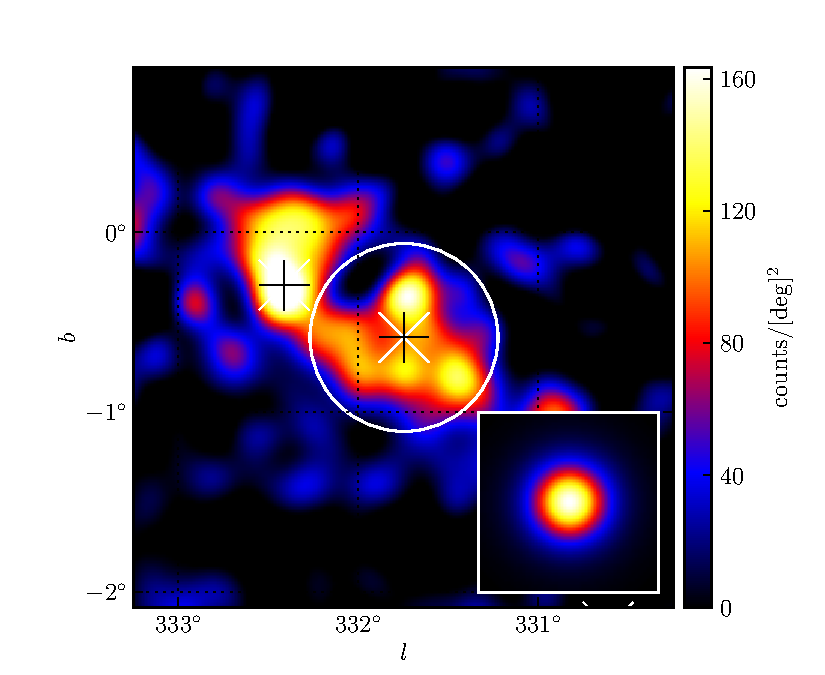
\includegraphics[type=pdf,ext=.pdf,read=.pdf]{source_plots/source_1FGL_J1613.6-5100c}
  \end{center}
  % this plot came from 
  % /u/gl/lande/work/fermi/extended_catalog/2FGL/plots_for_paper/source_plots/1FGL_J1613.6-5100c/v2/source_1FGL_J1613.6-5100c.pdf
  \caption{
    A galactic and isotropic diffuse subtracted 10 \gev to 100 \gev counts
    map of the region around 2FGL J1615.0-5051 and 2FGL J1615.2-5138
    smoothed by a 0.1\deg Gaussian kernel. The upper left source is
    2FGL J1615.0-5051 and the lower right source is 2FGL J1615.2-5138.
    The red stars are the catalog positions of these sources.  The red
    stars and circles are the best fit positions and extensions
    of these sources assuming uniform disk spatial model.  The green star
    inside of the extension of 2FGL J1615.2-5138  is 2FGL J1614.9-5212
    which was removed because it is part of the extended emission.
    The greeen stars to the left are 2FGL J1619.7-5040c and 2FGL
    J1620.6-5111c which were removed because they were not significant
    above 10\gev. These are shown as green stars.  The light blue contours
    are the \tev emission of
    the extended source HESS J1614-518 and the extended source HESS
    J1616-508 measured by H.E.S.S.(\cite{HESS_plane_survey}). 2FGL
    J1615.0-5051 is spatially
    consistent with HESS J1616-508 and 2FGL J1615.2-5138 is spatially
    consistent with HESS J1614-518.  More information about 2FGL
    J1615.0-5051 can be found in section~\ref{section_2FGL_J1615.0-5051} and
    2FGL J1615.2-5138 in section~\ref{section_2FGL_J1615.2-5138}.
  }\label{1FGL_J1613.6-5100c}
\end{figure}

\begin{figure}
  \begin{center}
    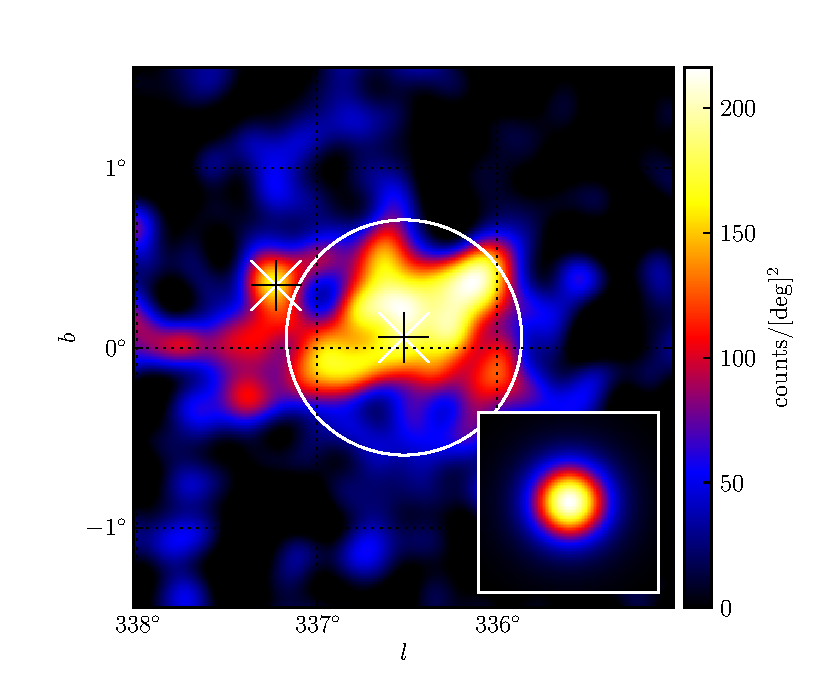
\includegraphics[type=pdf,ext=.pdf,read=.pdf]{source_plots/source_1FGL_J1632.9-4802c}
  \end{center}
  % this plot came from 
  % /u/gl/lande/work/fermi/extended_catalog/2FGL/plots_for_paper/source_plots/1FGL_J1632.9-4802c/v2/source_1FGL_J1632.9-4802c.pdf
  \caption{A galactic and isotropic diffuse subtracted 10 \gev to 100
  \gev counts map of the region around 2FGL J1632.4-4753c smoothed by
  a 0.1\deg Gaussian kernel.  This source is in a crowded region.
  The red star is the catalog position of this source.  The red
  cross and circle are the best fit position and extension 2FGL
  J1632.4-4753c assuming a uniform disk spatial model.  The three
  green crosses inside the extension are 2FGL
  J1631.7-4720c, 2FGL J1630.2-4752, and 2FGL J1634.4-4743c.4-4820c
  which were removed because they are part
  of the extended source.  The blue stars and crosses are the catalog
  positions and the relocalized positions of (from left to right)
  2FGL J1635.4-4717c and 2FGL J1636.3-4740c.  The farther away green
  stars are other catalog sources which were removed 
  because they are not significant
  above 10 \gev.  This extended source is spatially coincident
  with the extended H.E.S.S source HESS J1634-472.  The light blue
  contours are the \tev emission seen by H.E.S.S. 
  (\cite{HESS_plane_survey}). More information about this source 
  can be found in section~\ref{section_2FGL_J1632.4-4753c}.
  }\label{1FGL_J1632.9-4802c}
\end{figure}


\begin{figure}
  \begin{center}
    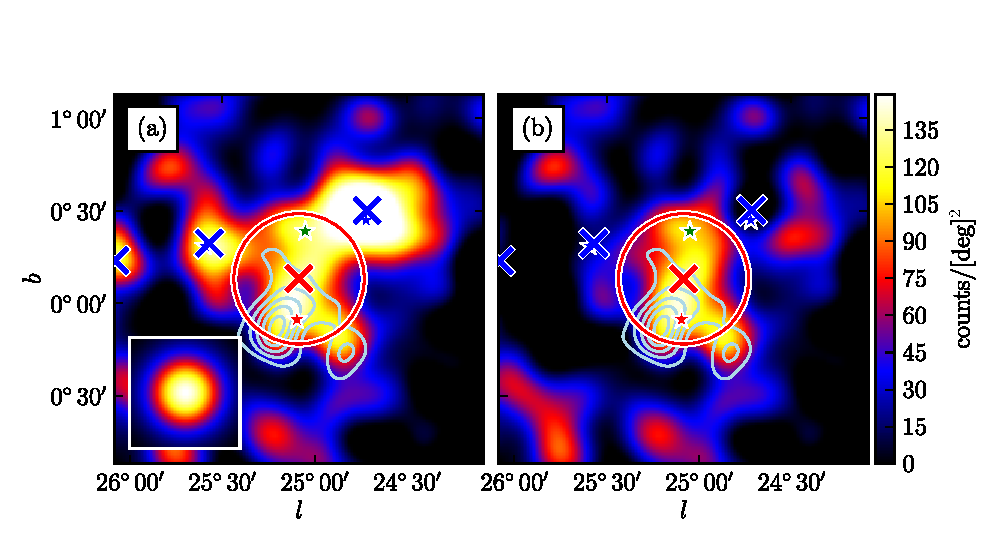
\includegraphics[type=pdf,ext=.pdf,read=.pdf]{source_plots/source_1FGL_J1837.5-0659c}
  \end{center}
  % this plot came from 
  % /u/gl/lande/work/fermi/extended_catalog/2FGL/plots_for_paper/source_plots/1FGL_J1837.5-0659c/v2/source_1FGL_J1837.5-0659c.pdf
  \caption{
  A galactic and isotropic diffuse subtracted 10 \gev to 100 \gev
  counts map of the region around 2FGL J1837.3-0700c smoothed by a
  0.1\deg Gaussian kernel.  The red star is the catalog position of
  this source. The red cross and circle are the best fit position and
  extension  of 2FGL J1837.3-0700c assuming a uniform disk spatial model.
  The blue stars and crosses are the catalog position and the relocalized
  position of (from left to right) 2FGL J1839.3-0558c, 2FGL J1836.8-0623c,
  and 2FGL J1834.7-0705c.  The green cross inside the extension is 
  2FGL J1835.5-0649 which was removed because it
  is part of the extended source.  The farther away green star is 2FGL
  J1839.0-0539 which was removed because it is not significant above
  10 \gev.  This source is spatially coincident with the \tev source HESS
  J1837-069.  The light blue contours are the \tev emission of HESS J1837-069
  observed by H.E.S.S (\cite{HESS_plane_survey}).  More information about
  this source can be found in section~\ref{section_2FGL_J1837.3-0700c}.
  }\label{1FGL_J1837.5-0659c}
\end{figure}


\begin{figure}
  \begin{center}
    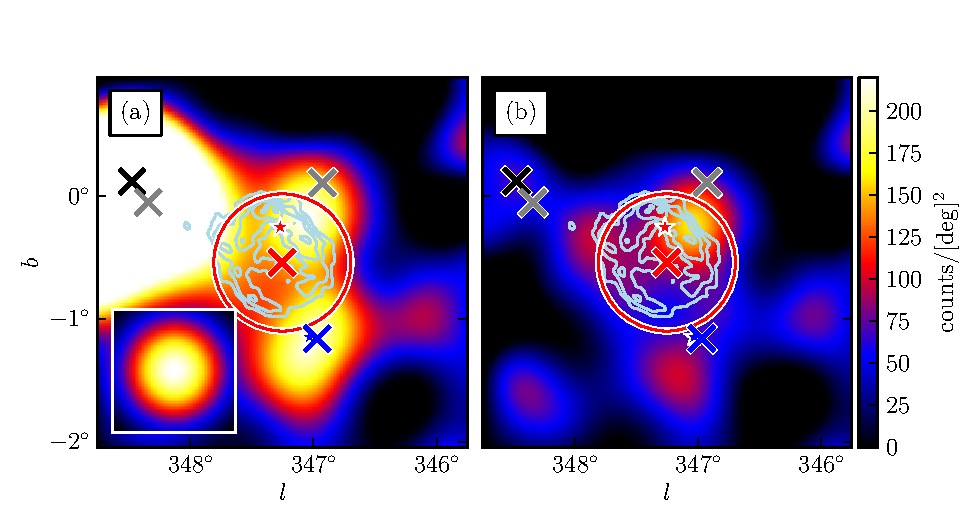
\includegraphics[type=pdf,ext=.pdf,read=.pdf]{source_plots/source_RX_J1713.7-3946}
    % this plot came from
  % /u/gl/lande/work/fermi/extended_catalog/2FGL/plots_for_paper/source_plots/RX_J1713.7-3946/v6/run.py
  \end{center}
  \caption{A galactic and isotropic diffuse subtracted 1 \gev to 100
  \gev counts map of the region around 2FGL J1712.4-3941 smoothed by a
  0.25\deg Gaussian kernel.  This source is spatially coincident with
  RX J1713.7-2946 was was recently reported by (\cite{rx_j1713_lat}).
  The light blue contours are the \tev emission reported by
  H.E.S.S. (\cite{rx_j1713_hess}).  The region was analyzed with the
  same background model as (\cite{rx_j1713_lat}).  Source A (blue cross)
  is spatially coincident with 2FGL J1715.4-4024c (blue star) so 2FGL
  J1715.4-4024c was moved to the position of source A.  The grey crosses
  represent from left to right the position of source B and C which were
  added to the background model. Plot (a) has the diffuse emisission model
  subtracted and plot (b) has the diffuse emission and all background
  sources also subtracted.
  }\label{2FGL_J1712.4-3941}
\end{figure}


\begin{figure}
  \begin{center}
    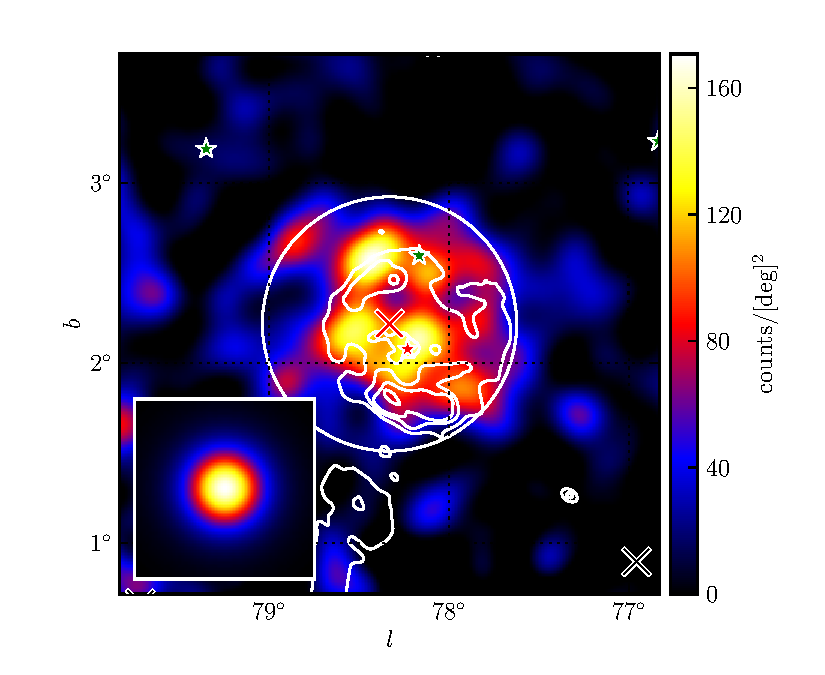
\includegraphics[type=pdf,ext=.pdf,read=.pdf]{source_plots/source_Gamma_Cygni}
  \end{center}
  % this plot came from 
  % /u/gl/lande/work/fermi/extended_catalog/2FGL/plots_for_paper/source_plots/Gamma_Cygni/v2/source_Gamma_Cygni.pdf
  \caption{A galactic and isotropic diffuse subtracted 10 \gev to 100
  \gev counts map of the region around 2FGL J2021.5+4026 smoothed by a
  0.1\deg Gaussian kernel. The red star is the catalog position of 2FGL
  J2021.5+4026.  The red cross and circle are the best fit position and
  extension 2FGL J2021.5+4026 assuming a uniform disk spatial model.
  The green cross inside the extension is 2FGL J2019.1+4040 which
  was removed because it is part of the extended source.  The farther
  away green stars represent other catalog sources which were removed
  because they were not significant above 10 \gev.  The grey cross is
  the position a source not in the two year catalog which was added
  to the region. 2FGL J2021.5+4026 is spatially coincident with the
  Gamma Cygni SNR.  The light blue contours are a 408MHz image of Gamma Cygni
  observed by the Canadian Galactic Plane Survey.  More information about
  this source can be found in section~\ref{section_2FGL J2021.5+4026}.
  }\label{1FGL_J2020.0+4049}
\end{figure}

\end{document}
